% Created by tikzDevice version 0.9 on 2016-01-10 21:46:33
% !TEX encoding = UTF-8 Unicode
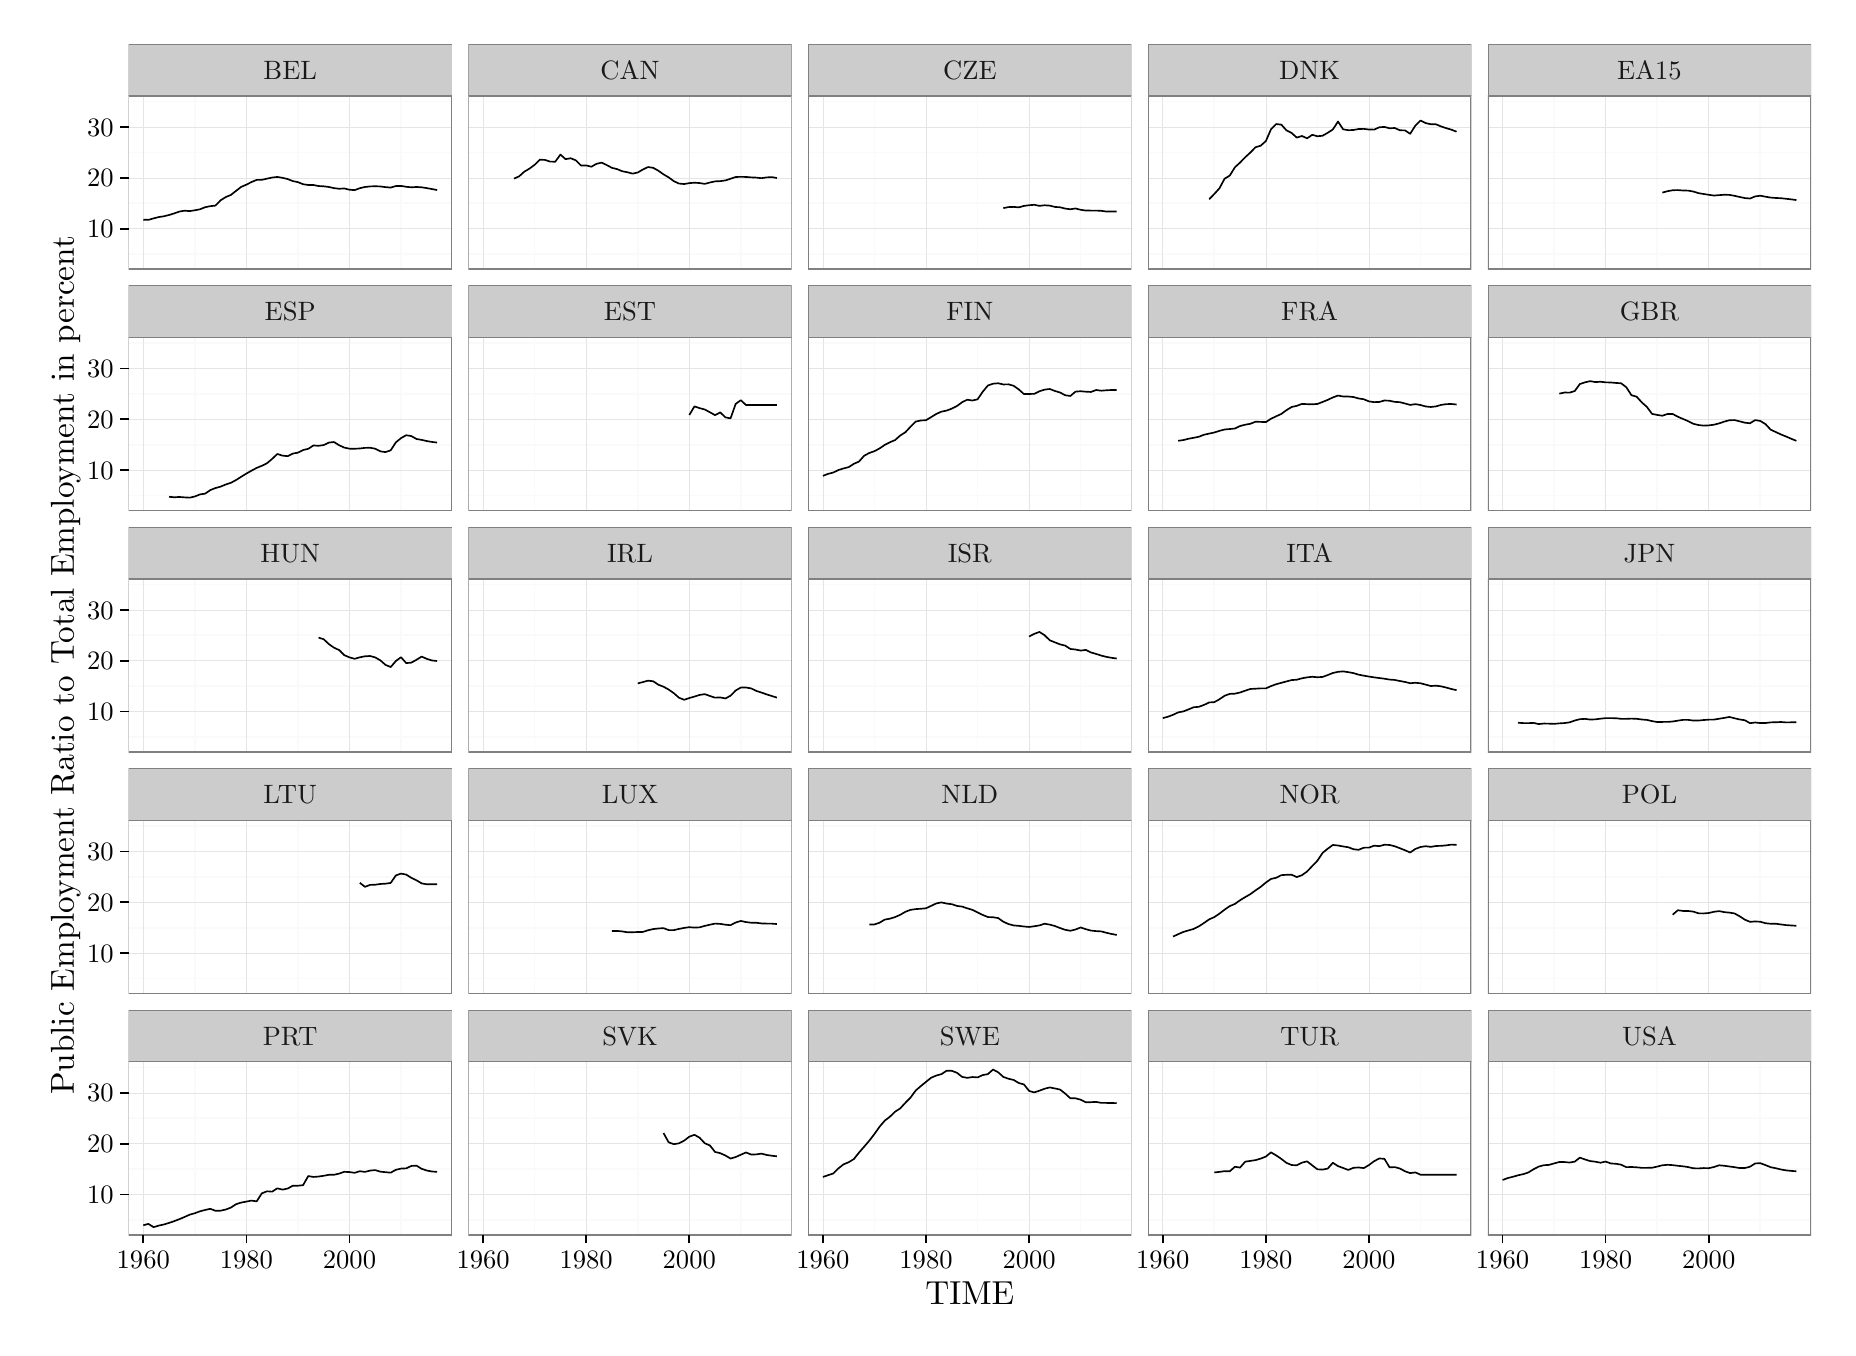
\begin{tikzpicture}[x=1pt,y=1pt]
\definecolor{fillColor}{RGB}{255,255,255}
\path[use as bounding box,fill=fillColor,fill opacity=0.00] (0,0) rectangle (650.43,469.75);
\begin{scope}
\path[clip] (  0.00,  0.00) rectangle (650.43,469.75);
\definecolor{drawColor}{RGB}{255,255,255}
\definecolor{fillColor}{RGB}{255,255,255}

\path[draw=drawColor,line width= 0.6pt,line join=round,line cap=round,fill=fillColor] (  0.00,  0.00) rectangle (650.43,469.76);
\end{scope}
\begin{scope}
\path[clip] ( 36.46,382.50) rectangle (153.26,445.14);
\definecolor{fillColor}{RGB}{255,255,255}

\path[fill=fillColor] ( 36.46,382.50) rectangle (153.26,445.14);
\definecolor{drawColor}{gray}{0.98}

\path[draw=drawColor,line width= 0.6pt,line join=round] ( 36.46,387.91) --
	(153.26,387.91);

\path[draw=drawColor,line width= 0.6pt,line join=round] ( 36.46,406.30) --
	(153.26,406.30);

\path[draw=drawColor,line width= 0.6pt,line join=round] ( 36.46,424.68) --
	(153.26,424.68);

\path[draw=drawColor,line width= 0.6pt,line join=round] ( 36.46,443.07) --
	(153.26,443.07);

\path[draw=drawColor,line width= 0.6pt,line join=round] ( 60.40,382.50) --
	( 60.40,445.14);

\path[draw=drawColor,line width= 0.6pt,line join=round] ( 97.65,382.50) --
	( 97.65,445.14);

\path[draw=drawColor,line width= 0.6pt,line join=round] (134.91,382.50) --
	(134.91,445.14);
\definecolor{drawColor}{gray}{0.90}

\path[draw=drawColor,line width= 0.2pt,line join=round] ( 36.46,397.11) --
	(153.26,397.11);

\path[draw=drawColor,line width= 0.2pt,line join=round] ( 36.46,415.49) --
	(153.26,415.49);

\path[draw=drawColor,line width= 0.2pt,line join=round] ( 36.46,433.88) --
	(153.26,433.88);

\path[draw=drawColor,line width= 0.2pt,line join=round] ( 41.77,382.50) --
	( 41.77,445.14);

\path[draw=drawColor,line width= 0.2pt,line join=round] ( 79.03,382.50) --
	( 79.03,445.14);

\path[draw=drawColor,line width= 0.2pt,line join=round] (116.28,382.50) --
	(116.28,445.14);
\definecolor{drawColor}{RGB}{0,0,0}

\path[draw=drawColor,line width= 0.6pt,line join=round] ( 41.77,400.35) --
	( 43.63,400.30) --
	( 45.50,400.83) --
	( 47.36,401.31) --
	( 49.22,401.59) --
	( 51.08,402.05) --
	( 52.95,402.63) --
	( 54.81,403.29) --
	( 56.67,403.62) --
	( 58.54,403.46) --
	( 60.40,403.76) --
	( 62.26,404.11) --
	( 64.12,404.87) --
	( 65.99,405.24) --
	( 67.85,405.45) --
	( 69.71,407.36) --
	( 71.57,408.53) --
	( 73.44,409.31) --
	( 75.30,410.78) --
	( 77.16,412.21) --
	( 79.03,413.02) --
	( 80.89,413.97) --
	( 82.75,414.74) --
	( 84.61,414.77) --
	( 86.48,415.18) --
	( 88.34,415.59) --
	( 90.20,415.80) --
	( 92.07,415.49) --
	( 93.93,415.05) --
	( 95.79,414.32) --
	( 97.65,413.92) --
	( 99.52,413.18) --
	(101.38,412.90) --
	(103.24,412.90) --
	(105.10,412.52) --
	(106.97,412.42) --
	(108.83,412.18) --
	(110.69,411.76) --
	(112.56,411.54) --
	(114.42,411.64) --
	(116.28,411.19) --
	(118.14,411.04) --
	(120.01,411.74) --
	(121.87,412.18) --
	(123.73,412.38) --
	(125.59,412.45) --
	(127.46,412.37) --
	(129.32,412.12) --
	(131.18,411.96) --
	(133.05,412.52) --
	(134.91,412.56) --
	(136.77,412.25) --
	(138.63,412.06) --
	(140.50,412.18) --
	(142.36,412.06) --
	(144.22,411.77) --
	(146.08,411.43) --
	(147.95,411.08);
\definecolor{drawColor}{gray}{0.50}

\path[draw=drawColor,line width= 0.6pt,line join=round,line cap=round] ( 36.46,382.50) rectangle (153.26,445.14);
\end{scope}
\begin{scope}
\path[clip] (159.26,382.50) rectangle (276.05,445.14);
\definecolor{fillColor}{RGB}{255,255,255}

\path[fill=fillColor] (159.26,382.50) rectangle (276.05,445.14);
\definecolor{drawColor}{gray}{0.98}

\path[draw=drawColor,line width= 0.6pt,line join=round] (159.26,387.91) --
	(276.05,387.91);

\path[draw=drawColor,line width= 0.6pt,line join=round] (159.26,406.30) --
	(276.05,406.30);

\path[draw=drawColor,line width= 0.6pt,line join=round] (159.26,424.68) --
	(276.05,424.68);

\path[draw=drawColor,line width= 0.6pt,line join=round] (159.26,443.07) --
	(276.05,443.07);

\path[draw=drawColor,line width= 0.6pt,line join=round] (183.19,382.50) --
	(183.19,445.14);

\path[draw=drawColor,line width= 0.6pt,line join=round] (220.45,382.50) --
	(220.45,445.14);

\path[draw=drawColor,line width= 0.6pt,line join=round] (257.70,382.50) --
	(257.70,445.14);
\definecolor{drawColor}{gray}{0.90}

\path[draw=drawColor,line width= 0.2pt,line join=round] (159.26,397.11) --
	(276.05,397.11);

\path[draw=drawColor,line width= 0.2pt,line join=round] (159.26,415.49) --
	(276.05,415.49);

\path[draw=drawColor,line width= 0.2pt,line join=round] (159.26,433.88) --
	(276.05,433.88);

\path[draw=drawColor,line width= 0.2pt,line join=round] (164.56,382.50) --
	(164.56,445.14);

\path[draw=drawColor,line width= 0.2pt,line join=round] (201.82,382.50) --
	(201.82,445.14);

\path[draw=drawColor,line width= 0.2pt,line join=round] (239.07,382.50) --
	(239.07,445.14);
\definecolor{drawColor}{RGB}{0,0,0}

\path[draw=drawColor,line width= 0.6pt,line join=round] (175.74,415.20) --
	(177.60,416.04) --
	(179.47,417.72) --
	(181.33,418.81) --
	(183.19,420.20) --
	(185.05,422.05) --
	(186.92,421.95) --
	(188.78,421.33) --
	(190.64,421.32) --
	(192.51,423.89) --
	(194.37,422.24) --
	(196.23,422.56) --
	(198.09,421.80) --
	(199.96,419.92) --
	(201.82,419.96) --
	(203.68,419.50) --
	(205.54,420.55) --
	(207.41,420.98) --
	(209.27,420.09) --
	(211.13,419.09) --
	(213.00,418.63) --
	(214.86,417.86) --
	(216.72,417.50) --
	(218.58,417.00) --
	(220.45,417.41) --
	(222.31,418.50) --
	(224.17,419.38) --
	(226.03,419.10) --
	(227.90,418.05) --
	(229.76,416.74) --
	(231.62,415.65) --
	(233.49,414.28) --
	(235.35,413.41) --
	(237.21,413.24) --
	(239.07,413.57) --
	(240.94,413.72) --
	(242.80,413.60) --
	(244.66,413.29) --
	(246.53,413.80) --
	(248.39,414.21) --
	(250.25,414.29) --
	(252.11,414.55) --
	(253.98,415.17) --
	(255.84,415.79) --
	(257.70,415.85) --
	(259.56,415.80) --
	(261.43,415.65) --
	(263.29,415.57) --
	(265.15,415.36) --
	(267.02,415.64) --
	(268.88,415.74) --
	(270.74,415.43);
\definecolor{drawColor}{gray}{0.50}

\path[draw=drawColor,line width= 0.6pt,line join=round,line cap=round] (159.26,382.50) rectangle (276.05,445.14);
\end{scope}
\begin{scope}
\path[clip] (282.05,382.50) rectangle (398.84,445.14);
\definecolor{fillColor}{RGB}{255,255,255}

\path[fill=fillColor] (282.05,382.50) rectangle (398.84,445.14);
\definecolor{drawColor}{gray}{0.98}

\path[draw=drawColor,line width= 0.6pt,line join=round] (282.05,387.91) --
	(398.84,387.91);

\path[draw=drawColor,line width= 0.6pt,line join=round] (282.05,406.30) --
	(398.84,406.30);

\path[draw=drawColor,line width= 0.6pt,line join=round] (282.05,424.68) --
	(398.84,424.68);

\path[draw=drawColor,line width= 0.6pt,line join=round] (282.05,443.07) --
	(398.84,443.07);

\path[draw=drawColor,line width= 0.6pt,line join=round] (305.99,382.50) --
	(305.99,445.14);

\path[draw=drawColor,line width= 0.6pt,line join=round] (343.24,382.50) --
	(343.24,445.14);

\path[draw=drawColor,line width= 0.6pt,line join=round] (380.49,382.50) --
	(380.49,445.14);
\definecolor{drawColor}{gray}{0.90}

\path[draw=drawColor,line width= 0.2pt,line join=round] (282.05,397.11) --
	(398.84,397.11);

\path[draw=drawColor,line width= 0.2pt,line join=round] (282.05,415.49) --
	(398.84,415.49);

\path[draw=drawColor,line width= 0.2pt,line join=round] (282.05,433.88) --
	(398.84,433.88);

\path[draw=drawColor,line width= 0.2pt,line join=round] (287.36,382.50) --
	(287.36,445.14);

\path[draw=drawColor,line width= 0.2pt,line join=round] (324.61,382.50) --
	(324.61,445.14);

\path[draw=drawColor,line width= 0.2pt,line join=round] (361.87,382.50) --
	(361.87,445.14);
\definecolor{drawColor}{RGB}{0,0,0}

\path[draw=drawColor,line width= 0.6pt,line join=round] (352.55,404.54) --
	(354.42,404.91) --
	(356.28,404.98) --
	(358.14,404.81) --
	(360.00,405.34) --
	(361.87,405.58) --
	(363.73,405.74) --
	(365.59,405.36) --
	(367.46,405.57) --
	(369.32,405.44) --
	(371.18,404.97) --
	(373.04,404.85) --
	(374.91,404.37) --
	(376.77,404.13) --
	(378.63,404.41) --
	(380.49,403.94) --
	(382.36,403.66) --
	(384.22,403.65) --
	(386.08,403.65) --
	(387.95,403.56) --
	(389.81,403.29) --
	(391.67,403.29) --
	(393.53,403.29);
\definecolor{drawColor}{gray}{0.50}

\path[draw=drawColor,line width= 0.6pt,line join=round,line cap=round] (282.05,382.50) rectangle (398.84,445.14);
\end{scope}
\begin{scope}
\path[clip] (404.84,382.50) rectangle (521.64,445.14);
\definecolor{fillColor}{RGB}{255,255,255}

\path[fill=fillColor] (404.84,382.50) rectangle (521.64,445.14);
\definecolor{drawColor}{gray}{0.98}

\path[draw=drawColor,line width= 0.6pt,line join=round] (404.84,387.91) --
	(521.64,387.91);

\path[draw=drawColor,line width= 0.6pt,line join=round] (404.84,406.30) --
	(521.64,406.30);

\path[draw=drawColor,line width= 0.6pt,line join=round] (404.84,424.68) --
	(521.64,424.68);

\path[draw=drawColor,line width= 0.6pt,line join=round] (404.84,443.07) --
	(521.64,443.07);

\path[draw=drawColor,line width= 0.6pt,line join=round] (428.78,382.50) --
	(428.78,445.14);

\path[draw=drawColor,line width= 0.6pt,line join=round] (466.03,382.50) --
	(466.03,445.14);

\path[draw=drawColor,line width= 0.6pt,line join=round] (503.29,382.50) --
	(503.29,445.14);
\definecolor{drawColor}{gray}{0.90}

\path[draw=drawColor,line width= 0.2pt,line join=round] (404.84,397.11) --
	(521.64,397.11);

\path[draw=drawColor,line width= 0.2pt,line join=round] (404.84,415.49) --
	(521.64,415.49);

\path[draw=drawColor,line width= 0.2pt,line join=round] (404.84,433.88) --
	(521.64,433.88);

\path[draw=drawColor,line width= 0.2pt,line join=round] (410.15,382.50) --
	(410.15,445.14);

\path[draw=drawColor,line width= 0.2pt,line join=round] (447.41,382.50) --
	(447.41,445.14);

\path[draw=drawColor,line width= 0.2pt,line join=round] (484.66,382.50) --
	(484.66,445.14);
\definecolor{drawColor}{RGB}{0,0,0}

\path[draw=drawColor,line width= 0.6pt,line join=round] (426.92,407.73) --
	(428.78,409.65) --
	(430.64,411.70) --
	(432.50,415.17) --
	(434.37,416.30) --
	(436.23,419.29) --
	(438.09,421.00) --
	(439.96,422.93) --
	(441.82,424.63) --
	(443.68,426.54) --
	(445.54,427.10) --
	(447.41,428.76) --
	(449.27,433.02) --
	(451.13,434.91) --
	(452.99,434.71) --
	(454.86,432.64) --
	(456.72,431.69) --
	(458.58,430.03) --
	(460.45,430.60) --
	(462.31,429.76) --
	(464.17,431.03) --
	(466.03,430.50) --
	(467.90,430.70) --
	(469.76,431.75) --
	(471.62,432.96) --
	(473.48,435.82) --
	(475.35,433.01) --
	(477.21,432.70) --
	(479.07,432.77) --
	(480.94,433.13) --
	(482.80,433.17) --
	(484.66,432.95) --
	(486.52,432.91) --
	(488.39,433.75) --
	(490.25,433.88) --
	(492.11,433.39) --
	(493.97,433.49) --
	(495.84,432.67) --
	(497.70,432.62) --
	(499.56,431.40) --
	(501.43,434.34) --
	(503.29,436.19) --
	(505.15,435.27) --
	(507.01,434.86) --
	(508.88,434.83) --
	(510.74,434.05) --
	(512.60,433.44) --
	(514.46,432.88) --
	(516.33,432.15);
\definecolor{drawColor}{gray}{0.50}

\path[draw=drawColor,line width= 0.6pt,line join=round,line cap=round] (404.84,382.50) rectangle (521.64,445.14);
\end{scope}
\begin{scope}
\path[clip] (527.64,382.50) rectangle (644.43,445.14);
\definecolor{fillColor}{RGB}{255,255,255}

\path[fill=fillColor] (527.64,382.50) rectangle (644.43,445.14);
\definecolor{drawColor}{gray}{0.98}

\path[draw=drawColor,line width= 0.6pt,line join=round] (527.64,387.91) --
	(644.43,387.91);

\path[draw=drawColor,line width= 0.6pt,line join=round] (527.64,406.30) --
	(644.43,406.30);

\path[draw=drawColor,line width= 0.6pt,line join=round] (527.64,424.68) --
	(644.43,424.68);

\path[draw=drawColor,line width= 0.6pt,line join=round] (527.64,443.07) --
	(644.43,443.07);

\path[draw=drawColor,line width= 0.6pt,line join=round] (551.57,382.50) --
	(551.57,445.14);

\path[draw=drawColor,line width= 0.6pt,line join=round] (588.83,382.50) --
	(588.83,445.14);

\path[draw=drawColor,line width= 0.6pt,line join=round] (626.08,382.50) --
	(626.08,445.14);
\definecolor{drawColor}{gray}{0.90}

\path[draw=drawColor,line width= 0.2pt,line join=round] (527.64,397.11) --
	(644.43,397.11);

\path[draw=drawColor,line width= 0.2pt,line join=round] (527.64,415.49) --
	(644.43,415.49);

\path[draw=drawColor,line width= 0.2pt,line join=round] (527.64,433.88) --
	(644.43,433.88);

\path[draw=drawColor,line width= 0.2pt,line join=round] (532.95,382.50) --
	(532.95,445.14);

\path[draw=drawColor,line width= 0.2pt,line join=round] (570.20,382.50) --
	(570.20,445.14);

\path[draw=drawColor,line width= 0.2pt,line join=round] (607.45,382.50) --
	(607.45,445.14);
\definecolor{drawColor}{RGB}{0,0,0}

\path[draw=drawColor,line width= 0.6pt,line join=round] (590.69,410.15) --
	(592.55,410.65) --
	(594.42,411.00) --
	(596.28,411.06) --
	(598.14,410.90) --
	(600.00,410.87) --
	(601.87,410.54) --
	(603.73,409.96) --
	(605.59,409.64) --
	(607.45,409.36) --
	(609.32,409.08) --
	(611.18,409.23) --
	(613.04,409.37) --
	(614.91,409.32) --
	(616.77,408.99) --
	(618.63,408.57) --
	(620.49,408.17) --
	(622.36,408.01) --
	(624.22,408.77) --
	(626.08,409.02) --
	(627.94,408.67) --
	(629.81,408.35) --
	(631.67,408.21) --
	(633.53,408.12) --
	(635.40,407.92) --
	(637.26,407.70) --
	(639.12,407.46);
\definecolor{drawColor}{gray}{0.50}

\path[draw=drawColor,line width= 0.6pt,line join=round,line cap=round] (527.64,382.50) rectangle (644.43,445.14);
\end{scope}
\begin{scope}
\path[clip] ( 36.46,295.24) rectangle (153.26,357.89);
\definecolor{fillColor}{RGB}{255,255,255}

\path[fill=fillColor] ( 36.46,295.24) rectangle (153.26,357.89);
\definecolor{drawColor}{gray}{0.98}

\path[draw=drawColor,line width= 0.6pt,line join=round] ( 36.46,300.66) --
	(153.26,300.66);

\path[draw=drawColor,line width= 0.6pt,line join=round] ( 36.46,319.04) --
	(153.26,319.04);

\path[draw=drawColor,line width= 0.6pt,line join=round] ( 36.46,337.43) --
	(153.26,337.43);

\path[draw=drawColor,line width= 0.6pt,line join=round] ( 36.46,355.81) --
	(153.26,355.81);

\path[draw=drawColor,line width= 0.6pt,line join=round] ( 60.40,295.24) --
	( 60.40,357.89);

\path[draw=drawColor,line width= 0.6pt,line join=round] ( 97.65,295.24) --
	( 97.65,357.89);

\path[draw=drawColor,line width= 0.6pt,line join=round] (134.91,295.24) --
	(134.91,357.89);
\definecolor{drawColor}{gray}{0.90}

\path[draw=drawColor,line width= 0.2pt,line join=round] ( 36.46,309.85) --
	(153.26,309.85);

\path[draw=drawColor,line width= 0.2pt,line join=round] ( 36.46,328.24) --
	(153.26,328.24);

\path[draw=drawColor,line width= 0.2pt,line join=round] ( 36.46,346.62) --
	(153.26,346.62);

\path[draw=drawColor,line width= 0.2pt,line join=round] ( 41.77,295.24) --
	( 41.77,357.89);

\path[draw=drawColor,line width= 0.2pt,line join=round] ( 79.03,295.24) --
	( 79.03,357.89);

\path[draw=drawColor,line width= 0.2pt,line join=round] (116.28,295.24) --
	(116.28,357.89);
\definecolor{drawColor}{RGB}{0,0,0}

\path[draw=drawColor,line width= 0.6pt,line join=round] ( 51.08,300.23) --
	( 52.95,300.06) --
	( 54.81,300.17) --
	( 56.67,300.02) --
	( 58.54,299.92) --
	( 60.40,300.34) --
	( 62.26,301.09) --
	( 64.12,301.36) --
	( 65.99,302.64) --
	( 67.85,303.39) --
	( 69.71,303.90) --
	( 71.57,304.68) --
	( 73.44,305.28) --
	( 75.30,306.29) --
	( 77.16,307.47) --
	( 79.03,308.62) --
	( 80.89,309.68) --
	( 82.75,310.67) --
	( 84.61,311.43) --
	( 86.48,312.36) --
	( 88.34,313.92) --
	( 90.20,315.70) --
	( 92.07,315.11) --
	( 93.93,314.91) --
	( 95.79,315.84) --
	( 97.65,316.18) --
	( 99.52,317.13) --
	(101.38,317.56) --
	(103.24,318.78) --
	(105.10,318.66) --
	(106.97,318.92) --
	(108.83,319.82) --
	(110.69,320.02) --
	(112.56,318.84) --
	(114.42,318.00) --
	(116.28,317.62) --
	(118.14,317.58) --
	(120.01,317.69) --
	(121.87,317.90) --
	(123.73,317.95) --
	(125.59,317.61) --
	(127.46,316.64) --
	(129.32,316.38) --
	(131.18,317.03) --
	(133.05,319.90) --
	(134.91,321.43) --
	(136.77,322.48) --
	(138.63,322.17) --
	(140.50,321.12) --
	(142.36,320.79) --
	(144.22,320.37) --
	(146.08,320.05) --
	(147.95,319.82);
\definecolor{drawColor}{gray}{0.50}

\path[draw=drawColor,line width= 0.6pt,line join=round,line cap=round] ( 36.46,295.24) rectangle (153.26,357.89);
\end{scope}
\begin{scope}
\path[clip] (159.26,295.24) rectangle (276.05,357.89);
\definecolor{fillColor}{RGB}{255,255,255}

\path[fill=fillColor] (159.26,295.24) rectangle (276.05,357.89);
\definecolor{drawColor}{gray}{0.98}

\path[draw=drawColor,line width= 0.6pt,line join=round] (159.26,300.66) --
	(276.05,300.66);

\path[draw=drawColor,line width= 0.6pt,line join=round] (159.26,319.04) --
	(276.05,319.04);

\path[draw=drawColor,line width= 0.6pt,line join=round] (159.26,337.43) --
	(276.05,337.43);

\path[draw=drawColor,line width= 0.6pt,line join=round] (159.26,355.81) --
	(276.05,355.81);

\path[draw=drawColor,line width= 0.6pt,line join=round] (183.19,295.24) --
	(183.19,357.89);

\path[draw=drawColor,line width= 0.6pt,line join=round] (220.45,295.24) --
	(220.45,357.89);

\path[draw=drawColor,line width= 0.6pt,line join=round] (257.70,295.24) --
	(257.70,357.89);
\definecolor{drawColor}{gray}{0.90}

\path[draw=drawColor,line width= 0.2pt,line join=round] (159.26,309.85) --
	(276.05,309.85);

\path[draw=drawColor,line width= 0.2pt,line join=round] (159.26,328.24) --
	(276.05,328.24);

\path[draw=drawColor,line width= 0.2pt,line join=round] (159.26,346.62) --
	(276.05,346.62);

\path[draw=drawColor,line width= 0.2pt,line join=round] (164.56,295.24) --
	(164.56,357.89);

\path[draw=drawColor,line width= 0.2pt,line join=round] (201.82,295.24) --
	(201.82,357.89);

\path[draw=drawColor,line width= 0.2pt,line join=round] (239.07,295.24) --
	(239.07,357.89);
\definecolor{drawColor}{RGB}{0,0,0}

\path[draw=drawColor,line width= 0.6pt,line join=round] (239.07,329.78) --
	(240.94,332.88) --
	(242.80,332.27) --
	(244.66,331.77) --
	(246.53,330.77) --
	(248.39,329.73) --
	(250.25,330.73) --
	(252.11,328.94) --
	(253.98,328.56) --
	(255.84,333.82) --
	(257.70,335.13) --
	(259.56,333.39) --
	(261.43,333.39) --
	(263.29,333.39) --
	(265.15,333.39) --
	(267.02,333.39) --
	(268.88,333.39) --
	(270.74,333.39);
\definecolor{drawColor}{gray}{0.50}

\path[draw=drawColor,line width= 0.6pt,line join=round,line cap=round] (159.26,295.24) rectangle (276.05,357.89);
\end{scope}
\begin{scope}
\path[clip] (282.05,295.24) rectangle (398.84,357.89);
\definecolor{fillColor}{RGB}{255,255,255}

\path[fill=fillColor] (282.05,295.24) rectangle (398.84,357.89);
\definecolor{drawColor}{gray}{0.98}

\path[draw=drawColor,line width= 0.6pt,line join=round] (282.05,300.66) --
	(398.84,300.66);

\path[draw=drawColor,line width= 0.6pt,line join=round] (282.05,319.04) --
	(398.84,319.04);

\path[draw=drawColor,line width= 0.6pt,line join=round] (282.05,337.43) --
	(398.84,337.43);

\path[draw=drawColor,line width= 0.6pt,line join=round] (282.05,355.81) --
	(398.84,355.81);

\path[draw=drawColor,line width= 0.6pt,line join=round] (305.99,295.24) --
	(305.99,357.89);

\path[draw=drawColor,line width= 0.6pt,line join=round] (343.24,295.24) --
	(343.24,357.89);

\path[draw=drawColor,line width= 0.6pt,line join=round] (380.49,295.24) --
	(380.49,357.89);
\definecolor{drawColor}{gray}{0.90}

\path[draw=drawColor,line width= 0.2pt,line join=round] (282.05,309.85) --
	(398.84,309.85);

\path[draw=drawColor,line width= 0.2pt,line join=round] (282.05,328.24) --
	(398.84,328.24);

\path[draw=drawColor,line width= 0.2pt,line join=round] (282.05,346.62) --
	(398.84,346.62);

\path[draw=drawColor,line width= 0.2pt,line join=round] (287.36,295.24) --
	(287.36,357.89);

\path[draw=drawColor,line width= 0.2pt,line join=round] (324.61,295.24) --
	(324.61,357.89);

\path[draw=drawColor,line width= 0.2pt,line join=round] (361.87,295.24) --
	(361.87,357.89);
\definecolor{drawColor}{RGB}{0,0,0}

\path[draw=drawColor,line width= 0.6pt,line join=round] (287.36,307.80) --
	(289.22,308.51) --
	(291.08,308.99) --
	(292.95,309.89) --
	(294.81,310.48) --
	(296.67,310.95) --
	(298.53,312.14) --
	(300.40,312.97) --
	(302.26,315.06) --
	(304.12,316.07) --
	(305.99,316.71) --
	(307.85,317.72) --
	(309.71,318.99) --
	(311.57,319.94) --
	(313.44,320.73) --
	(315.30,322.38) --
	(317.16,323.55) --
	(319.02,325.55) --
	(320.89,327.41) --
	(322.75,327.81) --
	(324.61,327.90) --
	(326.48,329.03) --
	(328.34,330.17) --
	(330.20,331.01) --
	(332.06,331.38) --
	(333.93,332.09) --
	(335.79,333.02) --
	(337.65,334.40) --
	(339.51,335.31) --
	(341.38,335.02) --
	(343.24,335.44) --
	(345.10,338.18) --
	(346.97,340.44) --
	(348.83,341.10) --
	(350.69,341.25) --
	(352.55,340.82) --
	(354.42,340.87) --
	(356.28,340.33) --
	(358.14,339.02) --
	(360.00,337.35) --
	(361.87,337.39) --
	(363.73,337.42) --
	(365.59,338.37) --
	(367.46,338.95) --
	(369.32,339.18) --
	(371.18,338.47) --
	(373.04,337.91) --
	(374.91,336.93) --
	(376.77,336.65) --
	(378.63,338.23) --
	(380.49,338.37) --
	(382.36,338.21) --
	(384.22,338.11) --
	(386.08,338.82) --
	(387.95,338.57) --
	(389.81,338.72) --
	(391.67,338.82) --
	(393.53,338.82);
\definecolor{drawColor}{gray}{0.50}

\path[draw=drawColor,line width= 0.6pt,line join=round,line cap=round] (282.05,295.24) rectangle (398.84,357.89);
\end{scope}
\begin{scope}
\path[clip] (404.84,295.24) rectangle (521.64,357.89);
\definecolor{fillColor}{RGB}{255,255,255}

\path[fill=fillColor] (404.84,295.24) rectangle (521.64,357.89);
\definecolor{drawColor}{gray}{0.98}

\path[draw=drawColor,line width= 0.6pt,line join=round] (404.84,300.66) --
	(521.64,300.66);

\path[draw=drawColor,line width= 0.6pt,line join=round] (404.84,319.04) --
	(521.64,319.04);

\path[draw=drawColor,line width= 0.6pt,line join=round] (404.84,337.43) --
	(521.64,337.43);

\path[draw=drawColor,line width= 0.6pt,line join=round] (404.84,355.81) --
	(521.64,355.81);

\path[draw=drawColor,line width= 0.6pt,line join=round] (428.78,295.24) --
	(428.78,357.89);

\path[draw=drawColor,line width= 0.6pt,line join=round] (466.03,295.24) --
	(466.03,357.89);

\path[draw=drawColor,line width= 0.6pt,line join=round] (503.29,295.24) --
	(503.29,357.89);
\definecolor{drawColor}{gray}{0.90}

\path[draw=drawColor,line width= 0.2pt,line join=round] (404.84,309.85) --
	(521.64,309.85);

\path[draw=drawColor,line width= 0.2pt,line join=round] (404.84,328.24) --
	(521.64,328.24);

\path[draw=drawColor,line width= 0.2pt,line join=round] (404.84,346.62) --
	(521.64,346.62);

\path[draw=drawColor,line width= 0.2pt,line join=round] (410.15,295.24) --
	(410.15,357.89);

\path[draw=drawColor,line width= 0.2pt,line join=round] (447.41,295.24) --
	(447.41,357.89);

\path[draw=drawColor,line width= 0.2pt,line join=round] (484.66,295.24) --
	(484.66,357.89);
\definecolor{drawColor}{RGB}{0,0,0}

\path[draw=drawColor,line width= 0.6pt,line join=round] (415.74,320.47) --
	(417.60,320.73) --
	(419.47,321.20) --
	(421.33,321.55) --
	(423.19,321.92) --
	(425.05,322.65) --
	(426.92,323.06) --
	(428.78,323.46) --
	(430.64,324.06) --
	(432.50,324.54) --
	(434.37,324.72) --
	(436.23,324.90) --
	(438.09,325.80) --
	(439.96,326.28) --
	(441.82,326.62) --
	(443.68,327.35) --
	(445.54,327.30) --
	(447.41,327.22) --
	(449.27,328.43) --
	(451.13,329.31) --
	(452.99,330.17) --
	(454.86,331.53) --
	(456.72,332.68) --
	(458.58,333.09) --
	(460.45,333.80) --
	(462.31,333.70) --
	(464.17,333.65) --
	(466.03,333.78) --
	(467.90,334.49) --
	(469.76,335.25) --
	(471.62,336.13) --
	(473.48,336.81) --
	(475.35,336.47) --
	(477.21,336.45) --
	(479.07,336.28) --
	(480.94,335.76) --
	(482.80,335.48) --
	(484.66,334.70) --
	(486.52,334.44) --
	(488.39,334.49) --
	(490.25,335.03) --
	(492.11,334.94) --
	(493.97,334.53) --
	(495.84,334.42) --
	(497.70,333.94) --
	(499.56,333.42) --
	(501.43,333.71) --
	(503.29,333.40) --
	(505.15,332.87) --
	(507.01,332.68) --
	(508.88,332.89) --
	(510.74,333.43) --
	(512.60,333.72) --
	(514.46,333.75) --
	(516.33,333.58);
\definecolor{drawColor}{gray}{0.50}

\path[draw=drawColor,line width= 0.6pt,line join=round,line cap=round] (404.84,295.24) rectangle (521.64,357.89);
\end{scope}
\begin{scope}
\path[clip] (527.64,295.24) rectangle (644.43,357.89);
\definecolor{fillColor}{RGB}{255,255,255}

\path[fill=fillColor] (527.64,295.24) rectangle (644.43,357.89);
\definecolor{drawColor}{gray}{0.98}

\path[draw=drawColor,line width= 0.6pt,line join=round] (527.64,300.66) --
	(644.43,300.66);

\path[draw=drawColor,line width= 0.6pt,line join=round] (527.64,319.04) --
	(644.43,319.04);

\path[draw=drawColor,line width= 0.6pt,line join=round] (527.64,337.43) --
	(644.43,337.43);

\path[draw=drawColor,line width= 0.6pt,line join=round] (527.64,355.81) --
	(644.43,355.81);

\path[draw=drawColor,line width= 0.6pt,line join=round] (551.57,295.24) --
	(551.57,357.89);

\path[draw=drawColor,line width= 0.6pt,line join=round] (588.83,295.24) --
	(588.83,357.89);

\path[draw=drawColor,line width= 0.6pt,line join=round] (626.08,295.24) --
	(626.08,357.89);
\definecolor{drawColor}{gray}{0.90}

\path[draw=drawColor,line width= 0.2pt,line join=round] (527.64,309.85) --
	(644.43,309.85);

\path[draw=drawColor,line width= 0.2pt,line join=round] (527.64,328.24) --
	(644.43,328.24);

\path[draw=drawColor,line width= 0.2pt,line join=round] (527.64,346.62) --
	(644.43,346.62);

\path[draw=drawColor,line width= 0.2pt,line join=round] (532.95,295.24) --
	(532.95,357.89);

\path[draw=drawColor,line width= 0.2pt,line join=round] (570.20,295.24) --
	(570.20,357.89);

\path[draw=drawColor,line width= 0.2pt,line join=round] (607.45,295.24) --
	(607.45,357.89);
\definecolor{drawColor}{RGB}{0,0,0}

\path[draw=drawColor,line width= 0.6pt,line join=round] (553.44,337.50) --
	(555.30,337.90) --
	(557.16,337.87) --
	(559.02,338.44) --
	(560.89,340.99) --
	(562.75,341.60) --
	(564.61,342.02) --
	(566.47,341.68) --
	(568.34,341.80) --
	(570.20,341.59) --
	(572.06,341.53) --
	(573.93,341.37) --
	(575.79,341.24) --
	(577.65,339.83) --
	(579.51,336.94) --
	(581.38,336.41) --
	(583.24,334.36) --
	(585.10,332.70) --
	(586.96,330.19) --
	(588.83,329.81) --
	(590.69,329.52) --
	(592.55,330.16) --
	(594.42,330.15) --
	(596.28,329.16) --
	(598.14,328.36) --
	(600.00,327.57) --
	(601.87,326.61) --
	(603.73,326.16) --
	(605.59,325.95) --
	(607.45,326.03) --
	(609.32,326.28) --
	(611.18,326.76) --
	(613.04,327.39) --
	(614.91,327.89) --
	(616.77,327.95) --
	(618.63,327.49) --
	(620.49,327.01) --
	(622.36,326.80) --
	(624.22,327.95) --
	(626.08,327.63) --
	(627.94,326.51) --
	(629.81,324.49) --
	(631.67,323.63) --
	(633.53,322.76) --
	(635.40,322.01) --
	(637.26,321.20) --
	(639.12,320.44);
\definecolor{drawColor}{gray}{0.50}

\path[draw=drawColor,line width= 0.6pt,line join=round,line cap=round] (527.64,295.24) rectangle (644.43,357.89);
\end{scope}
\begin{scope}
\path[clip] ( 36.46,207.99) rectangle (153.26,270.63);
\definecolor{fillColor}{RGB}{255,255,255}

\path[fill=fillColor] ( 36.46,207.99) rectangle (153.26,270.63);
\definecolor{drawColor}{gray}{0.98}

\path[draw=drawColor,line width= 0.6pt,line join=round] ( 36.46,213.40) --
	(153.26,213.40);

\path[draw=drawColor,line width= 0.6pt,line join=round] ( 36.46,231.79) --
	(153.26,231.79);

\path[draw=drawColor,line width= 0.6pt,line join=round] ( 36.46,250.17) --
	(153.26,250.17);

\path[draw=drawColor,line width= 0.6pt,line join=round] ( 36.46,268.56) --
	(153.26,268.56);

\path[draw=drawColor,line width= 0.6pt,line join=round] ( 60.40,207.99) --
	( 60.40,270.63);

\path[draw=drawColor,line width= 0.6pt,line join=round] ( 97.65,207.99) --
	( 97.65,270.63);

\path[draw=drawColor,line width= 0.6pt,line join=round] (134.91,207.99) --
	(134.91,270.63);
\definecolor{drawColor}{gray}{0.90}

\path[draw=drawColor,line width= 0.2pt,line join=round] ( 36.46,222.59) --
	(153.26,222.59);

\path[draw=drawColor,line width= 0.2pt,line join=round] ( 36.46,240.98) --
	(153.26,240.98);

\path[draw=drawColor,line width= 0.2pt,line join=round] ( 36.46,259.37) --
	(153.26,259.37);

\path[draw=drawColor,line width= 0.2pt,line join=round] ( 41.77,207.99) --
	( 41.77,270.63);

\path[draw=drawColor,line width= 0.2pt,line join=round] ( 79.03,207.99) --
	( 79.03,270.63);

\path[draw=drawColor,line width= 0.2pt,line join=round] (116.28,207.99) --
	(116.28,270.63);
\definecolor{drawColor}{RGB}{0,0,0}

\path[draw=drawColor,line width= 0.6pt,line join=round] (105.10,249.34) --
	(106.97,248.76) --
	(108.83,247.00) --
	(110.69,245.70) --
	(112.56,244.84) --
	(114.42,242.99) --
	(116.28,242.21) --
	(118.14,241.69) --
	(120.01,242.23) --
	(121.87,242.59) --
	(123.73,242.70) --
	(125.59,242.19) --
	(127.46,241.11) --
	(129.32,239.48) --
	(131.18,238.71) --
	(133.05,240.90) --
	(134.91,242.27) --
	(136.77,240.14) --
	(138.63,240.30) --
	(140.50,241.33) --
	(142.36,242.50) --
	(144.22,241.66) --
	(146.08,241.08) --
	(147.95,240.90);
\definecolor{drawColor}{gray}{0.50}

\path[draw=drawColor,line width= 0.6pt,line join=round,line cap=round] ( 36.46,207.99) rectangle (153.26,270.63);
\end{scope}
\begin{scope}
\path[clip] (159.26,207.99) rectangle (276.05,270.63);
\definecolor{fillColor}{RGB}{255,255,255}

\path[fill=fillColor] (159.26,207.99) rectangle (276.05,270.63);
\definecolor{drawColor}{gray}{0.98}

\path[draw=drawColor,line width= 0.6pt,line join=round] (159.26,213.40) --
	(276.05,213.40);

\path[draw=drawColor,line width= 0.6pt,line join=round] (159.26,231.79) --
	(276.05,231.79);

\path[draw=drawColor,line width= 0.6pt,line join=round] (159.26,250.17) --
	(276.05,250.17);

\path[draw=drawColor,line width= 0.6pt,line join=round] (159.26,268.56) --
	(276.05,268.56);

\path[draw=drawColor,line width= 0.6pt,line join=round] (183.19,207.99) --
	(183.19,270.63);

\path[draw=drawColor,line width= 0.6pt,line join=round] (220.45,207.99) --
	(220.45,270.63);

\path[draw=drawColor,line width= 0.6pt,line join=round] (257.70,207.99) --
	(257.70,270.63);
\definecolor{drawColor}{gray}{0.90}

\path[draw=drawColor,line width= 0.2pt,line join=round] (159.26,222.59) --
	(276.05,222.59);

\path[draw=drawColor,line width= 0.2pt,line join=round] (159.26,240.98) --
	(276.05,240.98);

\path[draw=drawColor,line width= 0.2pt,line join=round] (159.26,259.37) --
	(276.05,259.37);

\path[draw=drawColor,line width= 0.2pt,line join=round] (164.56,207.99) --
	(164.56,270.63);

\path[draw=drawColor,line width= 0.2pt,line join=round] (201.82,207.99) --
	(201.82,270.63);

\path[draw=drawColor,line width= 0.2pt,line join=round] (239.07,207.99) --
	(239.07,270.63);
\definecolor{drawColor}{RGB}{0,0,0}

\path[draw=drawColor,line width= 0.6pt,line join=round] (220.45,232.80) --
	(222.31,233.28) --
	(224.17,233.79) --
	(226.03,233.57) --
	(227.90,232.32) --
	(229.76,231.61) --
	(231.62,230.57) --
	(233.49,229.26) --
	(235.35,227.62) --
	(237.21,226.89) --
	(239.07,227.51) --
	(240.94,228.04) --
	(242.80,228.63) --
	(244.66,228.92) --
	(246.53,228.26) --
	(248.39,227.65) --
	(250.25,227.73) --
	(252.11,227.36) --
	(253.98,228.35) --
	(255.84,230.25) --
	(257.70,231.31) --
	(259.56,231.31) --
	(261.43,230.99) --
	(263.29,230.08) --
	(265.15,229.50) --
	(267.02,228.83) --
	(268.88,228.25) --
	(270.74,227.65);
\definecolor{drawColor}{gray}{0.50}

\path[draw=drawColor,line width= 0.6pt,line join=round,line cap=round] (159.26,207.99) rectangle (276.05,270.63);
\end{scope}
\begin{scope}
\path[clip] (282.05,207.99) rectangle (398.84,270.63);
\definecolor{fillColor}{RGB}{255,255,255}

\path[fill=fillColor] (282.05,207.99) rectangle (398.84,270.63);
\definecolor{drawColor}{gray}{0.98}

\path[draw=drawColor,line width= 0.6pt,line join=round] (282.05,213.40) --
	(398.84,213.40);

\path[draw=drawColor,line width= 0.6pt,line join=round] (282.05,231.79) --
	(398.84,231.79);

\path[draw=drawColor,line width= 0.6pt,line join=round] (282.05,250.17) --
	(398.84,250.17);

\path[draw=drawColor,line width= 0.6pt,line join=round] (282.05,268.56) --
	(398.84,268.56);

\path[draw=drawColor,line width= 0.6pt,line join=round] (305.99,207.99) --
	(305.99,270.63);

\path[draw=drawColor,line width= 0.6pt,line join=round] (343.24,207.99) --
	(343.24,270.63);

\path[draw=drawColor,line width= 0.6pt,line join=round] (380.49,207.99) --
	(380.49,270.63);
\definecolor{drawColor}{gray}{0.90}

\path[draw=drawColor,line width= 0.2pt,line join=round] (282.05,222.59) --
	(398.84,222.59);

\path[draw=drawColor,line width= 0.2pt,line join=round] (282.05,240.98) --
	(398.84,240.98);

\path[draw=drawColor,line width= 0.2pt,line join=round] (282.05,259.37) --
	(398.84,259.37);

\path[draw=drawColor,line width= 0.2pt,line join=round] (287.36,207.99) --
	(287.36,270.63);

\path[draw=drawColor,line width= 0.2pt,line join=round] (324.61,207.99) --
	(324.61,270.63);

\path[draw=drawColor,line width= 0.2pt,line join=round] (361.87,207.99) --
	(361.87,270.63);
\definecolor{drawColor}{RGB}{0,0,0}

\path[draw=drawColor,line width= 0.6pt,line join=round] (361.87,249.74) --
	(363.73,250.70) --
	(365.59,251.39) --
	(367.46,250.21) --
	(369.32,248.38) --
	(371.18,247.63) --
	(373.04,246.91) --
	(374.91,246.45) --
	(376.77,245.24) --
	(378.63,245.05) --
	(380.49,244.66) --
	(382.36,244.90) --
	(384.22,243.98) --
	(386.08,243.45) --
	(387.95,242.84) --
	(389.81,242.38) --
	(391.67,242.04) --
	(393.53,241.79);
\definecolor{drawColor}{gray}{0.50}

\path[draw=drawColor,line width= 0.6pt,line join=round,line cap=round] (282.05,207.99) rectangle (398.84,270.63);
\end{scope}
\begin{scope}
\path[clip] (404.84,207.99) rectangle (521.64,270.63);
\definecolor{fillColor}{RGB}{255,255,255}

\path[fill=fillColor] (404.84,207.99) rectangle (521.64,270.63);
\definecolor{drawColor}{gray}{0.98}

\path[draw=drawColor,line width= 0.6pt,line join=round] (404.84,213.40) --
	(521.64,213.40);

\path[draw=drawColor,line width= 0.6pt,line join=round] (404.84,231.79) --
	(521.64,231.79);

\path[draw=drawColor,line width= 0.6pt,line join=round] (404.84,250.17) --
	(521.64,250.17);

\path[draw=drawColor,line width= 0.6pt,line join=round] (404.84,268.56) --
	(521.64,268.56);

\path[draw=drawColor,line width= 0.6pt,line join=round] (428.78,207.99) --
	(428.78,270.63);

\path[draw=drawColor,line width= 0.6pt,line join=round] (466.03,207.99) --
	(466.03,270.63);

\path[draw=drawColor,line width= 0.6pt,line join=round] (503.29,207.99) --
	(503.29,270.63);
\definecolor{drawColor}{gray}{0.90}

\path[draw=drawColor,line width= 0.2pt,line join=round] (404.84,222.59) --
	(521.64,222.59);

\path[draw=drawColor,line width= 0.2pt,line join=round] (404.84,240.98) --
	(521.64,240.98);

\path[draw=drawColor,line width= 0.2pt,line join=round] (404.84,259.37) --
	(521.64,259.37);

\path[draw=drawColor,line width= 0.2pt,line join=round] (410.15,207.99) --
	(410.15,270.63);

\path[draw=drawColor,line width= 0.2pt,line join=round] (447.41,207.99) --
	(447.41,270.63);

\path[draw=drawColor,line width= 0.2pt,line join=round] (484.66,207.99) --
	(484.66,270.63);
\definecolor{drawColor}{RGB}{0,0,0}

\path[draw=drawColor,line width= 0.6pt,line join=round] (410.15,220.25) --
	(412.01,220.75) --
	(413.88,221.45) --
	(415.74,222.33) --
	(417.60,222.68) --
	(419.47,223.41) --
	(421.33,224.18) --
	(423.19,224.34) --
	(425.05,225.02) --
	(426.92,225.92) --
	(428.78,226.02) --
	(430.64,227.06) --
	(432.50,228.33) --
	(434.37,229.02) --
	(436.23,229.09) --
	(438.09,229.51) --
	(439.96,230.18) --
	(441.82,230.79) --
	(443.68,230.88) --
	(445.54,231.01) --
	(447.41,231.00) --
	(449.27,231.82) --
	(451.13,232.51) --
	(452.99,233.00) --
	(454.86,233.51) --
	(456.72,234.00) --
	(458.58,234.13) --
	(460.45,234.64) --
	(462.31,234.98) --
	(464.17,235.19) --
	(466.03,235.02) --
	(467.90,235.14) --
	(469.76,235.81) --
	(471.62,236.56) --
	(473.48,236.98) --
	(475.35,237.14) --
	(477.21,236.86) --
	(479.07,236.52) --
	(480.94,235.95) --
	(482.80,235.59) --
	(484.66,235.27) --
	(486.52,234.98) --
	(488.39,234.74) --
	(490.25,234.50) --
	(492.11,234.18) --
	(493.97,234.05) --
	(495.84,233.67) --
	(497.70,233.32) --
	(499.56,232.86) --
	(501.43,233.03) --
	(503.29,232.85) --
	(505.15,232.37) --
	(507.01,231.85) --
	(508.88,231.98) --
	(510.74,231.74) --
	(512.60,231.29) --
	(514.46,230.77) --
	(516.33,230.36);
\definecolor{drawColor}{gray}{0.50}

\path[draw=drawColor,line width= 0.6pt,line join=round,line cap=round] (404.84,207.99) rectangle (521.64,270.63);
\end{scope}
\begin{scope}
\path[clip] (527.64,207.99) rectangle (644.43,270.63);
\definecolor{fillColor}{RGB}{255,255,255}

\path[fill=fillColor] (527.64,207.99) rectangle (644.43,270.63);
\definecolor{drawColor}{gray}{0.98}

\path[draw=drawColor,line width= 0.6pt,line join=round] (527.64,213.40) --
	(644.43,213.40);

\path[draw=drawColor,line width= 0.6pt,line join=round] (527.64,231.79) --
	(644.43,231.79);

\path[draw=drawColor,line width= 0.6pt,line join=round] (527.64,250.17) --
	(644.43,250.17);

\path[draw=drawColor,line width= 0.6pt,line join=round] (527.64,268.56) --
	(644.43,268.56);

\path[draw=drawColor,line width= 0.6pt,line join=round] (551.57,207.99) --
	(551.57,270.63);

\path[draw=drawColor,line width= 0.6pt,line join=round] (588.83,207.99) --
	(588.83,270.63);

\path[draw=drawColor,line width= 0.6pt,line join=round] (626.08,207.99) --
	(626.08,270.63);
\definecolor{drawColor}{gray}{0.90}

\path[draw=drawColor,line width= 0.2pt,line join=round] (527.64,222.59) --
	(644.43,222.59);

\path[draw=drawColor,line width= 0.2pt,line join=round] (527.64,240.98) --
	(644.43,240.98);

\path[draw=drawColor,line width= 0.2pt,line join=round] (527.64,259.37) --
	(644.43,259.37);

\path[draw=drawColor,line width= 0.2pt,line join=round] (532.95,207.99) --
	(532.95,270.63);

\path[draw=drawColor,line width= 0.2pt,line join=round] (570.20,207.99) --
	(570.20,270.63);

\path[draw=drawColor,line width= 0.2pt,line join=round] (607.45,207.99) --
	(607.45,270.63);
\definecolor{drawColor}{RGB}{0,0,0}

\path[draw=drawColor,line width= 0.6pt,line join=round] (538.53,218.58) --
	(540.40,218.46) --
	(542.26,218.44) --
	(544.12,218.53) --
	(545.98,218.11) --
	(547.85,218.29) --
	(549.71,218.25) --
	(551.57,218.18) --
	(553.44,218.35) --
	(555.30,218.47) --
	(557.16,218.72) --
	(559.02,219.38) --
	(560.89,219.87) --
	(562.75,219.98) --
	(564.61,219.73) --
	(566.47,219.81) --
	(568.34,220.05) --
	(570.20,220.25) --
	(572.06,220.25) --
	(573.93,220.22) --
	(575.79,219.99) --
	(577.65,219.99) --
	(579.51,220.07) --
	(581.38,220.01) --
	(583.24,219.76) --
	(585.10,219.60) --
	(586.96,219.18) --
	(588.83,218.83) --
	(590.69,218.88) --
	(592.55,218.89) --
	(594.42,219.03) --
	(596.28,219.34) --
	(598.14,219.61) --
	(600.00,219.62) --
	(601.87,219.37) --
	(603.73,219.38) --
	(605.59,219.56) --
	(607.45,219.70) --
	(609.32,219.72) --
	(611.18,220.03) --
	(613.04,220.33) --
	(614.91,220.67) --
	(616.77,220.20) --
	(618.63,219.77) --
	(620.49,219.49) --
	(622.36,218.42) --
	(624.22,218.67) --
	(626.08,218.47) --
	(627.94,218.48) --
	(629.81,218.72) --
	(631.67,218.76) --
	(633.53,218.85) --
	(635.40,218.70) --
	(637.26,218.74) --
	(639.12,218.77);
\definecolor{drawColor}{gray}{0.50}

\path[draw=drawColor,line width= 0.6pt,line join=round,line cap=round] (527.64,207.99) rectangle (644.43,270.63);
\end{scope}
\begin{scope}
\path[clip] ( 36.46,120.73) rectangle (153.26,183.38);
\definecolor{fillColor}{RGB}{255,255,255}

\path[fill=fillColor] ( 36.46,120.73) rectangle (153.26,183.38);
\definecolor{drawColor}{gray}{0.98}

\path[draw=drawColor,line width= 0.6pt,line join=round] ( 36.46,126.15) --
	(153.26,126.15);

\path[draw=drawColor,line width= 0.6pt,line join=round] ( 36.46,144.53) --
	(153.26,144.53);

\path[draw=drawColor,line width= 0.6pt,line join=round] ( 36.46,162.92) --
	(153.26,162.92);

\path[draw=drawColor,line width= 0.6pt,line join=round] ( 36.46,181.30) --
	(153.26,181.30);

\path[draw=drawColor,line width= 0.6pt,line join=round] ( 60.40,120.73) --
	( 60.40,183.38);

\path[draw=drawColor,line width= 0.6pt,line join=round] ( 97.65,120.73) --
	( 97.65,183.38);

\path[draw=drawColor,line width= 0.6pt,line join=round] (134.91,120.73) --
	(134.91,183.38);
\definecolor{drawColor}{gray}{0.90}

\path[draw=drawColor,line width= 0.2pt,line join=round] ( 36.46,135.34) --
	(153.26,135.34);

\path[draw=drawColor,line width= 0.2pt,line join=round] ( 36.46,153.72) --
	(153.26,153.72);

\path[draw=drawColor,line width= 0.2pt,line join=round] ( 36.46,172.11) --
	(153.26,172.11);

\path[draw=drawColor,line width= 0.2pt,line join=round] ( 41.77,120.73) --
	( 41.77,183.38);

\path[draw=drawColor,line width= 0.2pt,line join=round] ( 79.03,120.73) --
	( 79.03,183.38);

\path[draw=drawColor,line width= 0.2pt,line join=round] (116.28,120.73) --
	(116.28,183.38);
\definecolor{drawColor}{RGB}{0,0,0}

\path[draw=drawColor,line width= 0.6pt,line join=round] (120.01,160.76) --
	(121.87,159.29) --
	(123.73,159.99) --
	(125.59,160.05) --
	(127.46,160.33) --
	(129.32,160.43) --
	(131.18,160.70) --
	(133.05,163.41) --
	(134.91,164.08) --
	(136.77,163.72) --
	(138.63,162.55) --
	(140.50,161.65) --
	(142.36,160.53) --
	(144.22,160.21) --
	(146.08,160.21) --
	(147.95,160.21);
\definecolor{drawColor}{gray}{0.50}

\path[draw=drawColor,line width= 0.6pt,line join=round,line cap=round] ( 36.46,120.73) rectangle (153.26,183.38);
\end{scope}
\begin{scope}
\path[clip] (159.26,120.73) rectangle (276.05,183.38);
\definecolor{fillColor}{RGB}{255,255,255}

\path[fill=fillColor] (159.26,120.73) rectangle (276.05,183.38);
\definecolor{drawColor}{gray}{0.98}

\path[draw=drawColor,line width= 0.6pt,line join=round] (159.26,126.15) --
	(276.05,126.15);

\path[draw=drawColor,line width= 0.6pt,line join=round] (159.26,144.53) --
	(276.05,144.53);

\path[draw=drawColor,line width= 0.6pt,line join=round] (159.26,162.92) --
	(276.05,162.92);

\path[draw=drawColor,line width= 0.6pt,line join=round] (159.26,181.30) --
	(276.05,181.30);

\path[draw=drawColor,line width= 0.6pt,line join=round] (183.19,120.73) --
	(183.19,183.38);

\path[draw=drawColor,line width= 0.6pt,line join=round] (220.45,120.73) --
	(220.45,183.38);

\path[draw=drawColor,line width= 0.6pt,line join=round] (257.70,120.73) --
	(257.70,183.38);
\definecolor{drawColor}{gray}{0.90}

\path[draw=drawColor,line width= 0.2pt,line join=round] (159.26,135.34) --
	(276.05,135.34);

\path[draw=drawColor,line width= 0.2pt,line join=round] (159.26,153.72) --
	(276.05,153.72);

\path[draw=drawColor,line width= 0.2pt,line join=round] (159.26,172.11) --
	(276.05,172.11);

\path[draw=drawColor,line width= 0.2pt,line join=round] (164.56,120.73) --
	(164.56,183.38);

\path[draw=drawColor,line width= 0.2pt,line join=round] (201.82,120.73) --
	(201.82,183.38);

\path[draw=drawColor,line width= 0.2pt,line join=round] (239.07,120.73) --
	(239.07,183.38);
\definecolor{drawColor}{RGB}{0,0,0}

\path[draw=drawColor,line width= 0.6pt,line join=round] (211.13,143.35) --
	(213.00,143.35) --
	(214.86,143.18) --
	(216.72,142.87) --
	(218.58,142.88) --
	(220.45,142.96) --
	(222.31,143.00) --
	(224.17,143.60) --
	(226.03,144.03) --
	(227.90,144.24) --
	(229.76,144.37) --
	(231.62,143.66) --
	(233.49,143.65) --
	(235.35,144.08) --
	(237.21,144.45) --
	(239.07,144.71) --
	(240.94,144.56) --
	(242.80,144.65) --
	(244.66,145.18) --
	(246.53,145.60) --
	(248.39,146.01) --
	(250.25,145.90) --
	(252.11,145.61) --
	(253.98,145.43) --
	(255.84,146.41) --
	(257.70,146.96) --
	(259.56,146.56) --
	(261.43,146.32) --
	(263.29,146.30) --
	(265.15,146.07) --
	(267.02,146.01) --
	(268.88,145.98) --
	(270.74,145.85);
\definecolor{drawColor}{gray}{0.50}

\path[draw=drawColor,line width= 0.6pt,line join=round,line cap=round] (159.26,120.73) rectangle (276.05,183.38);
\end{scope}
\begin{scope}
\path[clip] (282.05,120.73) rectangle (398.84,183.38);
\definecolor{fillColor}{RGB}{255,255,255}

\path[fill=fillColor] (282.05,120.73) rectangle (398.84,183.38);
\definecolor{drawColor}{gray}{0.98}

\path[draw=drawColor,line width= 0.6pt,line join=round] (282.05,126.15) --
	(398.84,126.15);

\path[draw=drawColor,line width= 0.6pt,line join=round] (282.05,144.53) --
	(398.84,144.53);

\path[draw=drawColor,line width= 0.6pt,line join=round] (282.05,162.92) --
	(398.84,162.92);

\path[draw=drawColor,line width= 0.6pt,line join=round] (282.05,181.30) --
	(398.84,181.30);

\path[draw=drawColor,line width= 0.6pt,line join=round] (305.99,120.73) --
	(305.99,183.38);

\path[draw=drawColor,line width= 0.6pt,line join=round] (343.24,120.73) --
	(343.24,183.38);

\path[draw=drawColor,line width= 0.6pt,line join=round] (380.49,120.73) --
	(380.49,183.38);
\definecolor{drawColor}{gray}{0.90}

\path[draw=drawColor,line width= 0.2pt,line join=round] (282.05,135.34) --
	(398.84,135.34);

\path[draw=drawColor,line width= 0.2pt,line join=round] (282.05,153.72) --
	(398.84,153.72);

\path[draw=drawColor,line width= 0.2pt,line join=round] (282.05,172.11) --
	(398.84,172.11);

\path[draw=drawColor,line width= 0.2pt,line join=round] (287.36,120.73) --
	(287.36,183.38);

\path[draw=drawColor,line width= 0.2pt,line join=round] (324.61,120.73) --
	(324.61,183.38);

\path[draw=drawColor,line width= 0.2pt,line join=round] (361.87,120.73) --
	(361.87,183.38);
\definecolor{drawColor}{RGB}{0,0,0}

\path[draw=drawColor,line width= 0.6pt,line join=round] (304.12,145.66) --
	(305.99,145.70) --
	(307.85,146.34) --
	(309.71,147.45) --
	(311.57,147.78) --
	(313.44,148.37) --
	(315.30,149.18) --
	(317.16,150.27) --
	(319.02,150.98) --
	(320.89,151.24) --
	(322.75,151.37) --
	(324.61,151.54) --
	(326.48,152.42) --
	(328.34,153.30) --
	(330.20,153.67) --
	(332.06,153.24) --
	(333.93,153.02) --
	(335.79,152.39) --
	(337.65,152.16) --
	(339.51,151.53) --
	(341.38,150.97) --
	(343.24,150.03) --
	(345.10,149.14) --
	(346.97,148.37) --
	(348.83,148.30) --
	(350.69,148.00) --
	(352.55,146.68) --
	(354.42,145.84) --
	(356.28,145.34) --
	(358.14,145.19) --
	(360.00,144.96) --
	(361.87,144.79) --
	(363.73,145.05) --
	(365.59,145.35) --
	(367.46,145.96) --
	(369.32,145.64) --
	(371.18,145.13) --
	(373.04,144.40) --
	(374.91,143.76) --
	(376.77,143.42) --
	(378.63,143.87) --
	(380.49,144.61) --
	(382.36,143.98) --
	(384.22,143.48) --
	(386.08,143.29) --
	(387.95,143.19) --
	(389.81,142.68) --
	(391.67,142.26) --
	(393.53,141.89);
\definecolor{drawColor}{gray}{0.50}

\path[draw=drawColor,line width= 0.6pt,line join=round,line cap=round] (282.05,120.73) rectangle (398.84,183.38);
\end{scope}
\begin{scope}
\path[clip] (404.84,120.73) rectangle (521.64,183.38);
\definecolor{fillColor}{RGB}{255,255,255}

\path[fill=fillColor] (404.84,120.73) rectangle (521.64,183.38);
\definecolor{drawColor}{gray}{0.98}

\path[draw=drawColor,line width= 0.6pt,line join=round] (404.84,126.15) --
	(521.64,126.15);

\path[draw=drawColor,line width= 0.6pt,line join=round] (404.84,144.53) --
	(521.64,144.53);

\path[draw=drawColor,line width= 0.6pt,line join=round] (404.84,162.92) --
	(521.64,162.92);

\path[draw=drawColor,line width= 0.6pt,line join=round] (404.84,181.30) --
	(521.64,181.30);

\path[draw=drawColor,line width= 0.6pt,line join=round] (428.78,120.73) --
	(428.78,183.38);

\path[draw=drawColor,line width= 0.6pt,line join=round] (466.03,120.73) --
	(466.03,183.38);

\path[draw=drawColor,line width= 0.6pt,line join=round] (503.29,120.73) --
	(503.29,183.38);
\definecolor{drawColor}{gray}{0.90}

\path[draw=drawColor,line width= 0.2pt,line join=round] (404.84,135.34) --
	(521.64,135.34);

\path[draw=drawColor,line width= 0.2pt,line join=round] (404.84,153.72) --
	(521.64,153.72);

\path[draw=drawColor,line width= 0.2pt,line join=round] (404.84,172.11) --
	(521.64,172.11);

\path[draw=drawColor,line width= 0.2pt,line join=round] (410.15,120.73) --
	(410.15,183.38);

\path[draw=drawColor,line width= 0.2pt,line join=round] (447.41,120.73) --
	(447.41,183.38);

\path[draw=drawColor,line width= 0.2pt,line join=round] (484.66,120.73) --
	(484.66,183.38);
\definecolor{drawColor}{RGB}{0,0,0}

\path[draw=drawColor,line width= 0.6pt,line join=round] (413.88,141.32) --
	(415.74,142.18) --
	(417.60,143.00) --
	(419.47,143.55) --
	(421.33,144.07) --
	(423.19,145.01) --
	(425.05,146.22) --
	(426.92,147.53) --
	(428.78,148.36) --
	(430.64,149.61) --
	(432.50,151.04) --
	(434.37,152.33) --
	(436.23,153.11) --
	(438.09,154.45) --
	(439.96,155.58) --
	(441.82,156.65) --
	(443.68,158.01) --
	(445.54,159.28) --
	(447.41,160.83) --
	(449.27,162.14) --
	(451.13,162.56) --
	(452.99,163.51) --
	(454.86,163.64) --
	(456.72,163.67) --
	(458.58,162.82) --
	(460.45,163.49) --
	(462.31,164.83) --
	(464.17,166.80) --
	(466.03,168.71) --
	(467.90,171.55) --
	(469.76,173.06) --
	(471.62,174.42) --
	(473.48,174.23) --
	(475.35,173.88) --
	(477.21,173.60) --
	(479.07,172.88) --
	(480.94,172.67) --
	(482.80,173.44) --
	(484.66,173.45) --
	(486.52,174.17) --
	(488.39,173.99) --
	(490.25,174.49) --
	(492.11,174.42) --
	(493.97,173.95) --
	(495.84,173.24) --
	(497.70,172.51) --
	(499.56,171.69) --
	(501.43,172.98) --
	(503.29,173.68) --
	(505.15,173.97) --
	(507.01,173.73) --
	(508.88,174.05) --
	(510.74,174.11) --
	(512.60,174.28) --
	(514.46,174.55) --
	(516.33,174.45);
\definecolor{drawColor}{gray}{0.50}

\path[draw=drawColor,line width= 0.6pt,line join=round,line cap=round] (404.84,120.73) rectangle (521.64,183.38);
\end{scope}
\begin{scope}
\path[clip] (527.64,120.73) rectangle (644.43,183.38);
\definecolor{fillColor}{RGB}{255,255,255}

\path[fill=fillColor] (527.64,120.73) rectangle (644.43,183.38);
\definecolor{drawColor}{gray}{0.98}

\path[draw=drawColor,line width= 0.6pt,line join=round] (527.64,126.15) --
	(644.43,126.15);

\path[draw=drawColor,line width= 0.6pt,line join=round] (527.64,144.53) --
	(644.43,144.53);

\path[draw=drawColor,line width= 0.6pt,line join=round] (527.64,162.92) --
	(644.43,162.92);

\path[draw=drawColor,line width= 0.6pt,line join=round] (527.64,181.30) --
	(644.43,181.30);

\path[draw=drawColor,line width= 0.6pt,line join=round] (551.57,120.73) --
	(551.57,183.38);

\path[draw=drawColor,line width= 0.6pt,line join=round] (588.83,120.73) --
	(588.83,183.38);

\path[draw=drawColor,line width= 0.6pt,line join=round] (626.08,120.73) --
	(626.08,183.38);
\definecolor{drawColor}{gray}{0.90}

\path[draw=drawColor,line width= 0.2pt,line join=round] (527.64,135.34) --
	(644.43,135.34);

\path[draw=drawColor,line width= 0.2pt,line join=round] (527.64,153.72) --
	(644.43,153.72);

\path[draw=drawColor,line width= 0.2pt,line join=round] (527.64,172.11) --
	(644.43,172.11);

\path[draw=drawColor,line width= 0.2pt,line join=round] (532.95,120.73) --
	(532.95,183.38);

\path[draw=drawColor,line width= 0.2pt,line join=round] (570.20,120.73) --
	(570.20,183.38);

\path[draw=drawColor,line width= 0.2pt,line join=round] (607.45,120.73) --
	(607.45,183.38);
\definecolor{drawColor}{RGB}{0,0,0}

\path[draw=drawColor,line width= 0.6pt,line join=round] (594.42,149.22) --
	(596.28,150.84) --
	(598.14,150.58) --
	(600.00,150.56) --
	(601.87,150.34) --
	(603.73,149.72) --
	(605.59,149.68) --
	(607.45,149.83) --
	(609.32,150.27) --
	(611.18,150.52) --
	(613.04,150.15) --
	(614.91,149.97) --
	(616.77,149.68) --
	(618.63,148.64) --
	(620.49,147.43) --
	(622.36,146.64) --
	(624.22,146.78) --
	(626.08,146.67) --
	(627.94,146.14) --
	(629.81,145.95) --
	(631.67,145.96) --
	(633.53,145.70) --
	(635.40,145.46) --
	(637.26,145.33) --
	(639.12,145.21);
\definecolor{drawColor}{gray}{0.50}

\path[draw=drawColor,line width= 0.6pt,line join=round,line cap=round] (527.64,120.73) rectangle (644.43,183.38);
\end{scope}
\begin{scope}
\path[clip] ( 36.46, 33.48) rectangle (153.26, 96.12);
\definecolor{fillColor}{RGB}{255,255,255}

\path[fill=fillColor] ( 36.46, 33.48) rectangle (153.26, 96.12);
\definecolor{drawColor}{gray}{0.98}

\path[draw=drawColor,line width= 0.6pt,line join=round] ( 36.46, 38.89) --
	(153.26, 38.89);

\path[draw=drawColor,line width= 0.6pt,line join=round] ( 36.46, 57.28) --
	(153.26, 57.28);

\path[draw=drawColor,line width= 0.6pt,line join=round] ( 36.46, 75.66) --
	(153.26, 75.66);

\path[draw=drawColor,line width= 0.6pt,line join=round] ( 36.46, 94.05) --
	(153.26, 94.05);

\path[draw=drawColor,line width= 0.6pt,line join=round] ( 60.40, 33.48) --
	( 60.40, 96.12);

\path[draw=drawColor,line width= 0.6pt,line join=round] ( 97.65, 33.48) --
	( 97.65, 96.12);

\path[draw=drawColor,line width= 0.6pt,line join=round] (134.91, 33.48) --
	(134.91, 96.12);
\definecolor{drawColor}{gray}{0.90}

\path[draw=drawColor,line width= 0.2pt,line join=round] ( 36.46, 48.08) --
	(153.26, 48.08);

\path[draw=drawColor,line width= 0.2pt,line join=round] ( 36.46, 66.47) --
	(153.26, 66.47);

\path[draw=drawColor,line width= 0.2pt,line join=round] ( 36.46, 84.85) --
	(153.26, 84.85);

\path[draw=drawColor,line width= 0.2pt,line join=round] ( 41.77, 33.48) --
	( 41.77, 96.12);

\path[draw=drawColor,line width= 0.2pt,line join=round] ( 79.03, 33.48) --
	( 79.03, 96.12);

\path[draw=drawColor,line width= 0.2pt,line join=round] (116.28, 33.48) --
	(116.28, 96.12);
\definecolor{drawColor}{RGB}{0,0,0}

\path[draw=drawColor,line width= 0.6pt,line join=round] ( 41.77, 37.01) --
	( 43.63, 37.49) --
	( 45.50, 36.32) --
	( 47.36, 36.88) --
	( 49.22, 37.28) --
	( 51.08, 37.85) --
	( 52.95, 38.49) --
	( 54.81, 39.20) --
	( 56.67, 39.98) --
	( 58.54, 40.83) --
	( 60.40, 41.35) --
	( 62.26, 42.04) --
	( 64.12, 42.53) --
	( 65.99, 42.95) --
	( 67.85, 42.23) --
	( 69.71, 42.27) --
	( 71.57, 42.68) --
	( 73.44, 43.39) --
	( 75.30, 44.61) --
	( 77.16, 45.20) --
	( 79.03, 45.55) --
	( 80.89, 45.92) --
	( 82.75, 45.63) --
	( 84.61, 48.54) --
	( 86.48, 49.27) --
	( 88.34, 49.14) --
	( 90.20, 50.35) --
	( 92.07, 49.88) --
	( 93.93, 50.26) --
	( 95.79, 51.28) --
	( 97.65, 51.29) --
	( 99.52, 51.48) --
	(101.38, 54.78) --
	(103.24, 54.46) --
	(105.10, 54.60) --
	(106.97, 54.88) --
	(108.83, 55.23) --
	(110.69, 55.24) --
	(112.56, 55.67) --
	(114.42, 56.32) --
	(116.28, 56.22) --
	(118.14, 55.95) --
	(120.01, 56.53) --
	(121.87, 56.28) --
	(123.73, 56.76) --
	(125.59, 56.93) --
	(127.46, 56.36) --
	(129.32, 56.18) --
	(131.18, 56.00) --
	(133.05, 57.04) --
	(134.91, 57.48) --
	(136.77, 57.56) --
	(138.63, 58.43) --
	(140.50, 58.55) --
	(142.36, 57.39) --
	(144.22, 56.77) --
	(146.08, 56.43) --
	(147.95, 56.29);
\definecolor{drawColor}{gray}{0.50}

\path[draw=drawColor,line width= 0.6pt,line join=round,line cap=round] ( 36.46, 33.48) rectangle (153.26, 96.12);
\end{scope}
\begin{scope}
\path[clip] (159.26, 33.48) rectangle (276.05, 96.12);
\definecolor{fillColor}{RGB}{255,255,255}

\path[fill=fillColor] (159.26, 33.48) rectangle (276.05, 96.12);
\definecolor{drawColor}{gray}{0.98}

\path[draw=drawColor,line width= 0.6pt,line join=round] (159.26, 38.89) --
	(276.05, 38.89);

\path[draw=drawColor,line width= 0.6pt,line join=round] (159.26, 57.28) --
	(276.05, 57.28);

\path[draw=drawColor,line width= 0.6pt,line join=round] (159.26, 75.66) --
	(276.05, 75.66);

\path[draw=drawColor,line width= 0.6pt,line join=round] (159.26, 94.05) --
	(276.05, 94.05);

\path[draw=drawColor,line width= 0.6pt,line join=round] (183.19, 33.48) --
	(183.19, 96.12);

\path[draw=drawColor,line width= 0.6pt,line join=round] (220.45, 33.48) --
	(220.45, 96.12);

\path[draw=drawColor,line width= 0.6pt,line join=round] (257.70, 33.48) --
	(257.70, 96.12);
\definecolor{drawColor}{gray}{0.90}

\path[draw=drawColor,line width= 0.2pt,line join=round] (159.26, 48.08) --
	(276.05, 48.08);

\path[draw=drawColor,line width= 0.2pt,line join=round] (159.26, 66.47) --
	(276.05, 66.47);

\path[draw=drawColor,line width= 0.2pt,line join=round] (159.26, 84.85) --
	(276.05, 84.85);

\path[draw=drawColor,line width= 0.2pt,line join=round] (164.56, 33.48) --
	(164.56, 96.12);

\path[draw=drawColor,line width= 0.2pt,line join=round] (201.82, 33.48) --
	(201.82, 96.12);

\path[draw=drawColor,line width= 0.2pt,line join=round] (239.07, 33.48) --
	(239.07, 96.12);
\definecolor{drawColor}{RGB}{0,0,0}

\path[draw=drawColor,line width= 0.6pt,line join=round] (229.76, 70.31) --
	(231.62, 66.97) --
	(233.49, 66.30) --
	(235.35, 66.61) --
	(237.21, 67.57) --
	(239.07, 69.01) --
	(240.94, 69.69) --
	(242.80, 68.63) --
	(244.66, 66.64) --
	(246.53, 65.83) --
	(248.39, 63.48) --
	(250.25, 63.05) --
	(252.11, 62.22) --
	(253.98, 61.11) --
	(255.84, 61.65) --
	(257.70, 62.50) --
	(259.56, 63.30) --
	(261.43, 62.55) --
	(263.29, 62.61) --
	(265.15, 62.89) --
	(267.02, 62.40) --
	(268.88, 62.13) --
	(270.74, 61.91);
\definecolor{drawColor}{gray}{0.50}

\path[draw=drawColor,line width= 0.6pt,line join=round,line cap=round] (159.26, 33.48) rectangle (276.05, 96.12);
\end{scope}
\begin{scope}
\path[clip] (282.05, 33.48) rectangle (398.84, 96.12);
\definecolor{fillColor}{RGB}{255,255,255}

\path[fill=fillColor] (282.05, 33.48) rectangle (398.84, 96.12);
\definecolor{drawColor}{gray}{0.98}

\path[draw=drawColor,line width= 0.6pt,line join=round] (282.05, 38.89) --
	(398.84, 38.89);

\path[draw=drawColor,line width= 0.6pt,line join=round] (282.05, 57.28) --
	(398.84, 57.28);

\path[draw=drawColor,line width= 0.6pt,line join=round] (282.05, 75.66) --
	(398.84, 75.66);

\path[draw=drawColor,line width= 0.6pt,line join=round] (282.05, 94.05) --
	(398.84, 94.05);

\path[draw=drawColor,line width= 0.6pt,line join=round] (305.99, 33.48) --
	(305.99, 96.12);

\path[draw=drawColor,line width= 0.6pt,line join=round] (343.24, 33.48) --
	(343.24, 96.12);

\path[draw=drawColor,line width= 0.6pt,line join=round] (380.49, 33.48) --
	(380.49, 96.12);
\definecolor{drawColor}{gray}{0.90}

\path[draw=drawColor,line width= 0.2pt,line join=round] (282.05, 48.08) --
	(398.84, 48.08);

\path[draw=drawColor,line width= 0.2pt,line join=round] (282.05, 66.47) --
	(398.84, 66.47);

\path[draw=drawColor,line width= 0.2pt,line join=round] (282.05, 84.85) --
	(398.84, 84.85);

\path[draw=drawColor,line width= 0.2pt,line join=round] (287.36, 33.48) --
	(287.36, 96.12);

\path[draw=drawColor,line width= 0.2pt,line join=round] (324.61, 33.48) --
	(324.61, 96.12);

\path[draw=drawColor,line width= 0.2pt,line join=round] (361.87, 33.48) --
	(361.87, 96.12);
\definecolor{drawColor}{RGB}{0,0,0}

\path[draw=drawColor,line width= 0.6pt,line join=round] (287.36, 54.45) --
	(289.22, 55.10) --
	(291.08, 55.69) --
	(292.95, 57.54) --
	(294.81, 59.01) --
	(296.67, 59.78) --
	(298.53, 60.92) --
	(300.40, 63.25) --
	(302.26, 65.40) --
	(304.12, 67.56) --
	(305.99, 70.00) --
	(307.85, 72.63) --
	(309.71, 74.81) --
	(311.57, 76.23) --
	(313.44, 78.03) --
	(315.30, 79.24) --
	(317.16, 81.26) --
	(319.02, 83.15) --
	(320.89, 85.69) --
	(322.75, 87.30) --
	(324.61, 88.82) --
	(326.48, 90.32) --
	(328.34, 91.10) --
	(330.20, 91.62) --
	(332.06, 92.86) --
	(333.93, 92.80) --
	(335.79, 92.10) --
	(337.65, 90.62) --
	(339.51, 90.26) --
	(341.38, 90.56) --
	(343.24, 90.43) --
	(345.10, 91.27) --
	(346.97, 91.62) --
	(348.83, 93.27) --
	(350.69, 92.27) --
	(352.55, 90.60) --
	(354.42, 89.94) --
	(356.28, 89.51) --
	(358.14, 88.40) --
	(360.00, 87.89) --
	(361.87, 85.54) --
	(363.73, 85.00) --
	(365.59, 85.63) --
	(367.46, 86.33) --
	(369.32, 86.81) --
	(371.18, 86.44) --
	(373.04, 86.04) --
	(374.91, 84.58) --
	(376.77, 82.87) --
	(378.63, 82.87) --
	(380.49, 82.38) --
	(382.36, 81.42) --
	(384.22, 81.48) --
	(386.08, 81.58) --
	(387.95, 81.22) --
	(389.81, 81.21) --
	(391.67, 81.17) --
	(393.53, 81.13);
\definecolor{drawColor}{gray}{0.50}

\path[draw=drawColor,line width= 0.6pt,line join=round,line cap=round] (282.05, 33.48) rectangle (398.84, 96.12);
\end{scope}
\begin{scope}
\path[clip] (404.84, 33.48) rectangle (521.64, 96.12);
\definecolor{fillColor}{RGB}{255,255,255}

\path[fill=fillColor] (404.84, 33.48) rectangle (521.64, 96.12);
\definecolor{drawColor}{gray}{0.98}

\path[draw=drawColor,line width= 0.6pt,line join=round] (404.84, 38.89) --
	(521.64, 38.89);

\path[draw=drawColor,line width= 0.6pt,line join=round] (404.84, 57.28) --
	(521.64, 57.28);

\path[draw=drawColor,line width= 0.6pt,line join=round] (404.84, 75.66) --
	(521.64, 75.66);

\path[draw=drawColor,line width= 0.6pt,line join=round] (404.84, 94.05) --
	(521.64, 94.05);

\path[draw=drawColor,line width= 0.6pt,line join=round] (428.78, 33.48) --
	(428.78, 96.12);

\path[draw=drawColor,line width= 0.6pt,line join=round] (466.03, 33.48) --
	(466.03, 96.12);

\path[draw=drawColor,line width= 0.6pt,line join=round] (503.29, 33.48) --
	(503.29, 96.12);
\definecolor{drawColor}{gray}{0.90}

\path[draw=drawColor,line width= 0.2pt,line join=round] (404.84, 48.08) --
	(521.64, 48.08);

\path[draw=drawColor,line width= 0.2pt,line join=round] (404.84, 66.47) --
	(521.64, 66.47);

\path[draw=drawColor,line width= 0.2pt,line join=round] (404.84, 84.85) --
	(521.64, 84.85);

\path[draw=drawColor,line width= 0.2pt,line join=round] (410.15, 33.48) --
	(410.15, 96.12);

\path[draw=drawColor,line width= 0.2pt,line join=round] (447.41, 33.48) --
	(447.41, 96.12);

\path[draw=drawColor,line width= 0.2pt,line join=round] (484.66, 33.48) --
	(484.66, 96.12);
\definecolor{drawColor}{RGB}{0,0,0}

\path[draw=drawColor,line width= 0.6pt,line join=round] (428.78, 56.08) --
	(430.64, 56.29) --
	(432.50, 56.55) --
	(434.37, 56.51) --
	(436.23, 58.14) --
	(438.09, 57.85) --
	(439.96, 59.99) --
	(441.82, 60.26) --
	(443.68, 60.54) --
	(445.54, 61.09) --
	(447.41, 61.82) --
	(449.27, 63.34) --
	(451.13, 62.25) --
	(452.99, 60.99) --
	(454.86, 59.54) --
	(456.72, 58.77) --
	(458.58, 58.66) --
	(460.45, 59.63) --
	(462.31, 60.09) --
	(464.17, 58.65) --
	(466.03, 57.22) --
	(467.90, 57.11) --
	(469.76, 57.47) --
	(471.62, 59.57) --
	(473.48, 58.38) --
	(475.35, 57.69) --
	(477.21, 56.98) --
	(479.07, 57.77) --
	(480.94, 57.88) --
	(482.80, 57.66) --
	(484.66, 58.75) --
	(486.52, 60.15) --
	(488.39, 61.13) --
	(490.25, 61.01) --
	(492.11, 57.92) --
	(493.97, 58.02) --
	(495.84, 57.51) --
	(497.70, 56.51) --
	(499.56, 55.84) --
	(501.43, 56.10) --
	(503.29, 55.27) --
	(505.15, 55.27) --
	(507.01, 55.27) --
	(508.88, 55.27) --
	(510.74, 55.27) --
	(512.60, 55.27) --
	(514.46, 55.27) --
	(516.33, 55.27);
\definecolor{drawColor}{gray}{0.50}

\path[draw=drawColor,line width= 0.6pt,line join=round,line cap=round] (404.84, 33.48) rectangle (521.64, 96.12);
\end{scope}
\begin{scope}
\path[clip] (527.64, 33.48) rectangle (644.43, 96.12);
\definecolor{fillColor}{RGB}{255,255,255}

\path[fill=fillColor] (527.64, 33.48) rectangle (644.43, 96.12);
\definecolor{drawColor}{gray}{0.98}

\path[draw=drawColor,line width= 0.6pt,line join=round] (527.64, 38.89) --
	(644.43, 38.89);

\path[draw=drawColor,line width= 0.6pt,line join=round] (527.64, 57.28) --
	(644.43, 57.28);

\path[draw=drawColor,line width= 0.6pt,line join=round] (527.64, 75.66) --
	(644.43, 75.66);

\path[draw=drawColor,line width= 0.6pt,line join=round] (527.64, 94.05) --
	(644.43, 94.05);

\path[draw=drawColor,line width= 0.6pt,line join=round] (551.57, 33.48) --
	(551.57, 96.12);

\path[draw=drawColor,line width= 0.6pt,line join=round] (588.83, 33.48) --
	(588.83, 96.12);

\path[draw=drawColor,line width= 0.6pt,line join=round] (626.08, 33.48) --
	(626.08, 96.12);
\definecolor{drawColor}{gray}{0.90}

\path[draw=drawColor,line width= 0.2pt,line join=round] (527.64, 48.08) --
	(644.43, 48.08);

\path[draw=drawColor,line width= 0.2pt,line join=round] (527.64, 66.47) --
	(644.43, 66.47);

\path[draw=drawColor,line width= 0.2pt,line join=round] (527.64, 84.85) --
	(644.43, 84.85);

\path[draw=drawColor,line width= 0.2pt,line join=round] (532.95, 33.48) --
	(532.95, 96.12);

\path[draw=drawColor,line width= 0.2pt,line join=round] (570.20, 33.48) --
	(570.20, 96.12);

\path[draw=drawColor,line width= 0.2pt,line join=round] (607.45, 33.48) --
	(607.45, 96.12);
\definecolor{drawColor}{RGB}{0,0,0}

\path[draw=drawColor,line width= 0.6pt,line join=round] (532.95, 53.36) --
	(534.81, 54.05) --
	(536.67, 54.52) --
	(538.53, 55.05) --
	(540.40, 55.47) --
	(542.26, 56.07) --
	(544.12, 57.23) --
	(545.98, 58.19) --
	(547.85, 58.70) --
	(549.71, 58.81) --
	(551.57, 59.35) --
	(553.44, 59.85) --
	(555.30, 59.84) --
	(557.16, 59.67) --
	(559.02, 59.99) --
	(560.89, 61.44) --
	(562.75, 60.77) --
	(564.61, 60.19) --
	(566.47, 59.97) --
	(568.34, 59.60) --
	(570.20, 60.02) --
	(572.06, 59.33) --
	(573.93, 59.22) --
	(575.79, 58.89) --
	(577.65, 57.99) --
	(579.51, 58.06) --
	(581.38, 57.94) --
	(583.24, 57.75) --
	(585.10, 57.75) --
	(586.96, 57.79) --
	(588.83, 58.20) --
	(590.69, 58.67) --
	(592.55, 58.85) --
	(594.42, 58.73) --
	(596.28, 58.49) --
	(598.14, 58.30) --
	(600.00, 58.03) --
	(601.87, 57.59) --
	(603.73, 57.54) --
	(605.59, 57.67) --
	(607.45, 57.62) --
	(609.32, 58.05) --
	(611.18, 58.67) --
	(613.04, 58.50) --
	(614.91, 58.24) --
	(616.77, 57.99) --
	(618.63, 57.67) --
	(620.49, 57.67) --
	(622.36, 58.16) --
	(624.22, 59.34) --
	(626.08, 59.43) --
	(627.94, 58.74) --
	(629.81, 57.98) --
	(631.67, 57.61) --
	(633.53, 57.16) --
	(635.40, 56.83) --
	(637.26, 56.65) --
	(639.12, 56.50);
\definecolor{drawColor}{gray}{0.50}

\path[draw=drawColor,line width= 0.6pt,line join=round,line cap=round] (527.64, 33.48) rectangle (644.43, 96.12);
\end{scope}
\begin{scope}
\path[clip] ( 36.46,445.14) rectangle (153.26,463.75);
\definecolor{drawColor}{gray}{0.50}
\definecolor{fillColor}{gray}{0.80}

\path[draw=drawColor,line width= 0.2pt,line join=round,line cap=round,fill=fillColor] ( 36.46,445.14) rectangle (153.26,463.75);
\definecolor{drawColor}{gray}{0.10}

\node[text=drawColor,anchor=base,inner sep=0pt, outer sep=0pt, scale=  0.96] at ( 94.86,451.14) {BEL};
\end{scope}
\begin{scope}
\path[clip] (159.26,445.14) rectangle (276.05,463.75);
\definecolor{drawColor}{gray}{0.50}
\definecolor{fillColor}{gray}{0.80}

\path[draw=drawColor,line width= 0.2pt,line join=round,line cap=round,fill=fillColor] (159.26,445.14) rectangle (276.05,463.75);
\definecolor{drawColor}{gray}{0.10}

\node[text=drawColor,anchor=base,inner sep=0pt, outer sep=0pt, scale=  0.96] at (217.65,451.14) {CAN};
\end{scope}
\begin{scope}
\path[clip] (282.05,445.14) rectangle (398.84,463.75);
\definecolor{drawColor}{gray}{0.50}
\definecolor{fillColor}{gray}{0.80}

\path[draw=drawColor,line width= 0.2pt,line join=round,line cap=round,fill=fillColor] (282.05,445.14) rectangle (398.84,463.75);
\definecolor{drawColor}{gray}{0.10}

\node[text=drawColor,anchor=base,inner sep=0pt, outer sep=0pt, scale=  0.96] at (340.45,451.14) {CZE};
\end{scope}
\begin{scope}
\path[clip] (404.84,445.14) rectangle (521.64,463.75);
\definecolor{drawColor}{gray}{0.50}
\definecolor{fillColor}{gray}{0.80}

\path[draw=drawColor,line width= 0.2pt,line join=round,line cap=round,fill=fillColor] (404.84,445.14) rectangle (521.64,463.75);
\definecolor{drawColor}{gray}{0.10}

\node[text=drawColor,anchor=base,inner sep=0pt, outer sep=0pt, scale=  0.96] at (463.24,451.14) {DNK};
\end{scope}
\begin{scope}
\path[clip] (527.64,445.14) rectangle (644.43,463.75);
\definecolor{drawColor}{gray}{0.50}
\definecolor{fillColor}{gray}{0.80}

\path[draw=drawColor,line width= 0.2pt,line join=round,line cap=round,fill=fillColor] (527.64,445.14) rectangle (644.43,463.75);
\definecolor{drawColor}{gray}{0.10}

\node[text=drawColor,anchor=base,inner sep=0pt, outer sep=0pt, scale=  0.96] at (586.03,451.14) {EA15};
\end{scope}
\begin{scope}
\path[clip] ( 36.46,357.89) rectangle (153.26,376.50);
\definecolor{drawColor}{gray}{0.50}
\definecolor{fillColor}{gray}{0.80}

\path[draw=drawColor,line width= 0.2pt,line join=round,line cap=round,fill=fillColor] ( 36.46,357.89) rectangle (153.26,376.50);
\definecolor{drawColor}{gray}{0.10}

\node[text=drawColor,anchor=base,inner sep=0pt, outer sep=0pt, scale=  0.96] at ( 94.86,363.89) {ESP};
\end{scope}
\begin{scope}
\path[clip] (159.26,357.89) rectangle (276.05,376.50);
\definecolor{drawColor}{gray}{0.50}
\definecolor{fillColor}{gray}{0.80}

\path[draw=drawColor,line width= 0.2pt,line join=round,line cap=round,fill=fillColor] (159.26,357.89) rectangle (276.05,376.50);
\definecolor{drawColor}{gray}{0.10}

\node[text=drawColor,anchor=base,inner sep=0pt, outer sep=0pt, scale=  0.96] at (217.65,363.89) {EST};
\end{scope}
\begin{scope}
\path[clip] (282.05,357.89) rectangle (398.84,376.50);
\definecolor{drawColor}{gray}{0.50}
\definecolor{fillColor}{gray}{0.80}

\path[draw=drawColor,line width= 0.2pt,line join=round,line cap=round,fill=fillColor] (282.05,357.89) rectangle (398.84,376.50);
\definecolor{drawColor}{gray}{0.10}

\node[text=drawColor,anchor=base,inner sep=0pt, outer sep=0pt, scale=  0.96] at (340.45,363.89) {FIN};
\end{scope}
\begin{scope}
\path[clip] (404.84,357.89) rectangle (521.64,376.50);
\definecolor{drawColor}{gray}{0.50}
\definecolor{fillColor}{gray}{0.80}

\path[draw=drawColor,line width= 0.2pt,line join=round,line cap=round,fill=fillColor] (404.84,357.89) rectangle (521.64,376.50);
\definecolor{drawColor}{gray}{0.10}

\node[text=drawColor,anchor=base,inner sep=0pt, outer sep=0pt, scale=  0.96] at (463.24,363.89) {FRA};
\end{scope}
\begin{scope}
\path[clip] (527.64,357.89) rectangle (644.43,376.50);
\definecolor{drawColor}{gray}{0.50}
\definecolor{fillColor}{gray}{0.80}

\path[draw=drawColor,line width= 0.2pt,line join=round,line cap=round,fill=fillColor] (527.64,357.89) rectangle (644.43,376.50);
\definecolor{drawColor}{gray}{0.10}

\node[text=drawColor,anchor=base,inner sep=0pt, outer sep=0pt, scale=  0.96] at (586.03,363.89) {GBR};
\end{scope}
\begin{scope}
\path[clip] ( 36.46,270.63) rectangle (153.26,289.24);
\definecolor{drawColor}{gray}{0.50}
\definecolor{fillColor}{gray}{0.80}

\path[draw=drawColor,line width= 0.2pt,line join=round,line cap=round,fill=fillColor] ( 36.46,270.63) rectangle (153.26,289.24);
\definecolor{drawColor}{gray}{0.10}

\node[text=drawColor,anchor=base,inner sep=0pt, outer sep=0pt, scale=  0.96] at ( 94.86,276.63) {HUN};
\end{scope}
\begin{scope}
\path[clip] (159.26,270.63) rectangle (276.05,289.24);
\definecolor{drawColor}{gray}{0.50}
\definecolor{fillColor}{gray}{0.80}

\path[draw=drawColor,line width= 0.2pt,line join=round,line cap=round,fill=fillColor] (159.26,270.63) rectangle (276.05,289.24);
\definecolor{drawColor}{gray}{0.10}

\node[text=drawColor,anchor=base,inner sep=0pt, outer sep=0pt, scale=  0.96] at (217.65,276.63) {IRL};
\end{scope}
\begin{scope}
\path[clip] (282.05,270.63) rectangle (398.84,289.24);
\definecolor{drawColor}{gray}{0.50}
\definecolor{fillColor}{gray}{0.80}

\path[draw=drawColor,line width= 0.2pt,line join=round,line cap=round,fill=fillColor] (282.05,270.63) rectangle (398.84,289.24);
\definecolor{drawColor}{gray}{0.10}

\node[text=drawColor,anchor=base,inner sep=0pt, outer sep=0pt, scale=  0.96] at (340.45,276.63) {ISR};
\end{scope}
\begin{scope}
\path[clip] (404.84,270.63) rectangle (521.64,289.24);
\definecolor{drawColor}{gray}{0.50}
\definecolor{fillColor}{gray}{0.80}

\path[draw=drawColor,line width= 0.2pt,line join=round,line cap=round,fill=fillColor] (404.84,270.63) rectangle (521.64,289.24);
\definecolor{drawColor}{gray}{0.10}

\node[text=drawColor,anchor=base,inner sep=0pt, outer sep=0pt, scale=  0.96] at (463.24,276.63) {ITA};
\end{scope}
\begin{scope}
\path[clip] (527.64,270.63) rectangle (644.43,289.24);
\definecolor{drawColor}{gray}{0.50}
\definecolor{fillColor}{gray}{0.80}

\path[draw=drawColor,line width= 0.2pt,line join=round,line cap=round,fill=fillColor] (527.64,270.63) rectangle (644.43,289.24);
\definecolor{drawColor}{gray}{0.10}

\node[text=drawColor,anchor=base,inner sep=0pt, outer sep=0pt, scale=  0.96] at (586.03,276.63) {JPN};
\end{scope}
\begin{scope}
\path[clip] ( 36.46,183.38) rectangle (153.26,201.99);
\definecolor{drawColor}{gray}{0.50}
\definecolor{fillColor}{gray}{0.80}

\path[draw=drawColor,line width= 0.2pt,line join=round,line cap=round,fill=fillColor] ( 36.46,183.38) rectangle (153.26,201.99);
\definecolor{drawColor}{gray}{0.10}

\node[text=drawColor,anchor=base,inner sep=0pt, outer sep=0pt, scale=  0.96] at ( 94.86,189.38) {LTU};
\end{scope}
\begin{scope}
\path[clip] (159.26,183.38) rectangle (276.05,201.99);
\definecolor{drawColor}{gray}{0.50}
\definecolor{fillColor}{gray}{0.80}

\path[draw=drawColor,line width= 0.2pt,line join=round,line cap=round,fill=fillColor] (159.26,183.38) rectangle (276.05,201.99);
\definecolor{drawColor}{gray}{0.10}

\node[text=drawColor,anchor=base,inner sep=0pt, outer sep=0pt, scale=  0.96] at (217.65,189.38) {LUX};
\end{scope}
\begin{scope}
\path[clip] (282.05,183.38) rectangle (398.84,201.99);
\definecolor{drawColor}{gray}{0.50}
\definecolor{fillColor}{gray}{0.80}

\path[draw=drawColor,line width= 0.2pt,line join=round,line cap=round,fill=fillColor] (282.05,183.38) rectangle (398.84,201.99);
\definecolor{drawColor}{gray}{0.10}

\node[text=drawColor,anchor=base,inner sep=0pt, outer sep=0pt, scale=  0.96] at (340.45,189.38) {NLD};
\end{scope}
\begin{scope}
\path[clip] (404.84,183.38) rectangle (521.64,201.99);
\definecolor{drawColor}{gray}{0.50}
\definecolor{fillColor}{gray}{0.80}

\path[draw=drawColor,line width= 0.2pt,line join=round,line cap=round,fill=fillColor] (404.84,183.38) rectangle (521.64,201.99);
\definecolor{drawColor}{gray}{0.10}

\node[text=drawColor,anchor=base,inner sep=0pt, outer sep=0pt, scale=  0.96] at (463.24,189.38) {NOR};
\end{scope}
\begin{scope}
\path[clip] (527.64,183.38) rectangle (644.43,201.99);
\definecolor{drawColor}{gray}{0.50}
\definecolor{fillColor}{gray}{0.80}

\path[draw=drawColor,line width= 0.2pt,line join=round,line cap=round,fill=fillColor] (527.64,183.38) rectangle (644.43,201.99);
\definecolor{drawColor}{gray}{0.10}

\node[text=drawColor,anchor=base,inner sep=0pt, outer sep=0pt, scale=  0.96] at (586.03,189.38) {POL};
\end{scope}
\begin{scope}
\path[clip] ( 36.46, 96.12) rectangle (153.26,114.73);
\definecolor{drawColor}{gray}{0.50}
\definecolor{fillColor}{gray}{0.80}

\path[draw=drawColor,line width= 0.2pt,line join=round,line cap=round,fill=fillColor] ( 36.46, 96.12) rectangle (153.26,114.73);
\definecolor{drawColor}{gray}{0.10}

\node[text=drawColor,anchor=base,inner sep=0pt, outer sep=0pt, scale=  0.96] at ( 94.86,102.12) {PRT};
\end{scope}
\begin{scope}
\path[clip] (159.26, 96.12) rectangle (276.05,114.73);
\definecolor{drawColor}{gray}{0.50}
\definecolor{fillColor}{gray}{0.80}

\path[draw=drawColor,line width= 0.2pt,line join=round,line cap=round,fill=fillColor] (159.26, 96.12) rectangle (276.05,114.73);
\definecolor{drawColor}{gray}{0.10}

\node[text=drawColor,anchor=base,inner sep=0pt, outer sep=0pt, scale=  0.96] at (217.65,102.12) {SVK};
\end{scope}
\begin{scope}
\path[clip] (282.05, 96.12) rectangle (398.84,114.73);
\definecolor{drawColor}{gray}{0.50}
\definecolor{fillColor}{gray}{0.80}

\path[draw=drawColor,line width= 0.2pt,line join=round,line cap=round,fill=fillColor] (282.05, 96.12) rectangle (398.84,114.73);
\definecolor{drawColor}{gray}{0.10}

\node[text=drawColor,anchor=base,inner sep=0pt, outer sep=0pt, scale=  0.96] at (340.45,102.12) {SWE};
\end{scope}
\begin{scope}
\path[clip] (404.84, 96.12) rectangle (521.64,114.73);
\definecolor{drawColor}{gray}{0.50}
\definecolor{fillColor}{gray}{0.80}

\path[draw=drawColor,line width= 0.2pt,line join=round,line cap=round,fill=fillColor] (404.84, 96.12) rectangle (521.64,114.73);
\definecolor{drawColor}{gray}{0.10}

\node[text=drawColor,anchor=base,inner sep=0pt, outer sep=0pt, scale=  0.96] at (463.24,102.12) {TUR};
\end{scope}
\begin{scope}
\path[clip] (527.64, 96.12) rectangle (644.43,114.73);
\definecolor{drawColor}{gray}{0.50}
\definecolor{fillColor}{gray}{0.80}

\path[draw=drawColor,line width= 0.2pt,line join=round,line cap=round,fill=fillColor] (527.64, 96.12) rectangle (644.43,114.73);
\definecolor{drawColor}{gray}{0.10}

\node[text=drawColor,anchor=base,inner sep=0pt, outer sep=0pt, scale=  0.96] at (586.03,102.12) {USA};
\end{scope}
\begin{scope}
\path[clip] (  0.00,  0.00) rectangle (650.43,469.75);
\definecolor{drawColor}{RGB}{0,0,0}

\node[text=drawColor,anchor=base east,inner sep=0pt, outer sep=0pt, scale=  0.96] at ( 31.06,393.80) {10};

\node[text=drawColor,anchor=base east,inner sep=0pt, outer sep=0pt, scale=  0.96] at ( 31.06,412.19) {20};

\node[text=drawColor,anchor=base east,inner sep=0pt, outer sep=0pt, scale=  0.96] at ( 31.06,430.57) {30};
\end{scope}
\begin{scope}
\path[clip] (  0.00,  0.00) rectangle (650.43,469.75);
\definecolor{drawColor}{RGB}{0,0,0}

\path[draw=drawColor,line width= 0.6pt,line join=round] ( 33.46,397.11) --
	( 36.46,397.11);

\path[draw=drawColor,line width= 0.6pt,line join=round] ( 33.46,415.49) --
	( 36.46,415.49);

\path[draw=drawColor,line width= 0.6pt,line join=round] ( 33.46,433.88) --
	( 36.46,433.88);
\end{scope}
\begin{scope}
\path[clip] (  0.00,  0.00) rectangle (650.43,469.75);
\definecolor{drawColor}{RGB}{0,0,0}

\node[text=drawColor,anchor=base east,inner sep=0pt, outer sep=0pt, scale=  0.96] at ( 31.06,306.54) {10};

\node[text=drawColor,anchor=base east,inner sep=0pt, outer sep=0pt, scale=  0.96] at ( 31.06,324.93) {20};

\node[text=drawColor,anchor=base east,inner sep=0pt, outer sep=0pt, scale=  0.96] at ( 31.06,343.32) {30};
\end{scope}
\begin{scope}
\path[clip] (  0.00,  0.00) rectangle (650.43,469.75);
\definecolor{drawColor}{RGB}{0,0,0}

\path[draw=drawColor,line width= 0.6pt,line join=round] ( 33.46,309.85) --
	( 36.46,309.85);

\path[draw=drawColor,line width= 0.6pt,line join=round] ( 33.46,328.24) --
	( 36.46,328.24);

\path[draw=drawColor,line width= 0.6pt,line join=round] ( 33.46,346.62) --
	( 36.46,346.62);
\end{scope}
\begin{scope}
\path[clip] (  0.00,  0.00) rectangle (650.43,469.75);
\definecolor{drawColor}{RGB}{0,0,0}

\node[text=drawColor,anchor=base east,inner sep=0pt, outer sep=0pt, scale=  0.96] at ( 31.06,219.29) {10};

\node[text=drawColor,anchor=base east,inner sep=0pt, outer sep=0pt, scale=  0.96] at ( 31.06,237.67) {20};

\node[text=drawColor,anchor=base east,inner sep=0pt, outer sep=0pt, scale=  0.96] at ( 31.06,256.06) {30};
\end{scope}
\begin{scope}
\path[clip] (  0.00,  0.00) rectangle (650.43,469.75);
\definecolor{drawColor}{RGB}{0,0,0}

\path[draw=drawColor,line width= 0.6pt,line join=round] ( 33.46,222.59) --
	( 36.46,222.59);

\path[draw=drawColor,line width= 0.6pt,line join=round] ( 33.46,240.98) --
	( 36.46,240.98);

\path[draw=drawColor,line width= 0.6pt,line join=round] ( 33.46,259.37) --
	( 36.46,259.37);
\end{scope}
\begin{scope}
\path[clip] (  0.00,  0.00) rectangle (650.43,469.75);
\definecolor{drawColor}{RGB}{0,0,0}

\node[text=drawColor,anchor=base east,inner sep=0pt, outer sep=0pt, scale=  0.96] at ( 31.06,132.03) {10};

\node[text=drawColor,anchor=base east,inner sep=0pt, outer sep=0pt, scale=  0.96] at ( 31.06,150.42) {20};

\node[text=drawColor,anchor=base east,inner sep=0pt, outer sep=0pt, scale=  0.96] at ( 31.06,168.80) {30};
\end{scope}
\begin{scope}
\path[clip] (  0.00,  0.00) rectangle (650.43,469.75);
\definecolor{drawColor}{RGB}{0,0,0}

\path[draw=drawColor,line width= 0.6pt,line join=round] ( 33.46,135.34) --
	( 36.46,135.34);

\path[draw=drawColor,line width= 0.6pt,line join=round] ( 33.46,153.72) --
	( 36.46,153.72);

\path[draw=drawColor,line width= 0.6pt,line join=round] ( 33.46,172.11) --
	( 36.46,172.11);
\end{scope}
\begin{scope}
\path[clip] (  0.00,  0.00) rectangle (650.43,469.75);
\definecolor{drawColor}{RGB}{0,0,0}

\node[text=drawColor,anchor=base east,inner sep=0pt, outer sep=0pt, scale=  0.96] at ( 31.06, 44.78) {10};

\node[text=drawColor,anchor=base east,inner sep=0pt, outer sep=0pt, scale=  0.96] at ( 31.06, 63.16) {20};

\node[text=drawColor,anchor=base east,inner sep=0pt, outer sep=0pt, scale=  0.96] at ( 31.06, 81.55) {30};
\end{scope}
\begin{scope}
\path[clip] (  0.00,  0.00) rectangle (650.43,469.75);
\definecolor{drawColor}{RGB}{0,0,0}

\path[draw=drawColor,line width= 0.6pt,line join=round] ( 33.46, 48.08) --
	( 36.46, 48.08);

\path[draw=drawColor,line width= 0.6pt,line join=round] ( 33.46, 66.47) --
	( 36.46, 66.47);

\path[draw=drawColor,line width= 0.6pt,line join=round] ( 33.46, 84.85) --
	( 36.46, 84.85);
\end{scope}
\begin{scope}
\path[clip] (  0.00,  0.00) rectangle (650.43,469.75);
\definecolor{drawColor}{RGB}{0,0,0}

\path[draw=drawColor,line width= 0.6pt,line join=round] ( 41.77, 30.48) --
	( 41.77, 33.48);

\path[draw=drawColor,line width= 0.6pt,line join=round] ( 79.03, 30.48) --
	( 79.03, 33.48);

\path[draw=drawColor,line width= 0.6pt,line join=round] (116.28, 30.48) --
	(116.28, 33.48);
\end{scope}
\begin{scope}
\path[clip] (  0.00,  0.00) rectangle (650.43,469.75);
\definecolor{drawColor}{RGB}{0,0,0}

\node[text=drawColor,anchor=base,inner sep=0pt, outer sep=0pt, scale=  0.96] at ( 41.77, 21.46) {1960};

\node[text=drawColor,anchor=base,inner sep=0pt, outer sep=0pt, scale=  0.96] at ( 79.03, 21.46) {1980};

\node[text=drawColor,anchor=base,inner sep=0pt, outer sep=0pt, scale=  0.96] at (116.28, 21.46) {2000};
\end{scope}
\begin{scope}
\path[clip] (  0.00,  0.00) rectangle (650.43,469.75);
\definecolor{drawColor}{RGB}{0,0,0}

\path[draw=drawColor,line width= 0.6pt,line join=round] (164.56, 30.48) --
	(164.56, 33.48);

\path[draw=drawColor,line width= 0.6pt,line join=round] (201.82, 30.48) --
	(201.82, 33.48);

\path[draw=drawColor,line width= 0.6pt,line join=round] (239.07, 30.48) --
	(239.07, 33.48);
\end{scope}
\begin{scope}
\path[clip] (  0.00,  0.00) rectangle (650.43,469.75);
\definecolor{drawColor}{RGB}{0,0,0}

\node[text=drawColor,anchor=base,inner sep=0pt, outer sep=0pt, scale=  0.96] at (164.56, 21.46) {1960};

\node[text=drawColor,anchor=base,inner sep=0pt, outer sep=0pt, scale=  0.96] at (201.82, 21.46) {1980};

\node[text=drawColor,anchor=base,inner sep=0pt, outer sep=0pt, scale=  0.96] at (239.07, 21.46) {2000};
\end{scope}
\begin{scope}
\path[clip] (  0.00,  0.00) rectangle (650.43,469.75);
\definecolor{drawColor}{RGB}{0,0,0}

\path[draw=drawColor,line width= 0.6pt,line join=round] (287.36, 30.48) --
	(287.36, 33.48);

\path[draw=drawColor,line width= 0.6pt,line join=round] (324.61, 30.48) --
	(324.61, 33.48);

\path[draw=drawColor,line width= 0.6pt,line join=round] (361.87, 30.48) --
	(361.87, 33.48);
\end{scope}
\begin{scope}
\path[clip] (  0.00,  0.00) rectangle (650.43,469.75);
\definecolor{drawColor}{RGB}{0,0,0}

\node[text=drawColor,anchor=base,inner sep=0pt, outer sep=0pt, scale=  0.96] at (287.36, 21.46) {1960};

\node[text=drawColor,anchor=base,inner sep=0pt, outer sep=0pt, scale=  0.96] at (324.61, 21.46) {1980};

\node[text=drawColor,anchor=base,inner sep=0pt, outer sep=0pt, scale=  0.96] at (361.87, 21.46) {2000};
\end{scope}
\begin{scope}
\path[clip] (  0.00,  0.00) rectangle (650.43,469.75);
\definecolor{drawColor}{RGB}{0,0,0}

\path[draw=drawColor,line width= 0.6pt,line join=round] (410.15, 30.48) --
	(410.15, 33.48);

\path[draw=drawColor,line width= 0.6pt,line join=round] (447.41, 30.48) --
	(447.41, 33.48);

\path[draw=drawColor,line width= 0.6pt,line join=round] (484.66, 30.48) --
	(484.66, 33.48);
\end{scope}
\begin{scope}
\path[clip] (  0.00,  0.00) rectangle (650.43,469.75);
\definecolor{drawColor}{RGB}{0,0,0}

\node[text=drawColor,anchor=base,inner sep=0pt, outer sep=0pt, scale=  0.96] at (410.15, 21.46) {1960};

\node[text=drawColor,anchor=base,inner sep=0pt, outer sep=0pt, scale=  0.96] at (447.41, 21.46) {1980};

\node[text=drawColor,anchor=base,inner sep=0pt, outer sep=0pt, scale=  0.96] at (484.66, 21.46) {2000};
\end{scope}
\begin{scope}
\path[clip] (  0.00,  0.00) rectangle (650.43,469.75);
\definecolor{drawColor}{RGB}{0,0,0}

\path[draw=drawColor,line width= 0.6pt,line join=round] (532.95, 30.48) --
	(532.95, 33.48);

\path[draw=drawColor,line width= 0.6pt,line join=round] (570.20, 30.48) --
	(570.20, 33.48);

\path[draw=drawColor,line width= 0.6pt,line join=round] (607.45, 30.48) --
	(607.45, 33.48);
\end{scope}
\begin{scope}
\path[clip] (  0.00,  0.00) rectangle (650.43,469.75);
\definecolor{drawColor}{RGB}{0,0,0}

\node[text=drawColor,anchor=base,inner sep=0pt, outer sep=0pt, scale=  0.96] at (532.95, 21.46) {1960};

\node[text=drawColor,anchor=base,inner sep=0pt, outer sep=0pt, scale=  0.96] at (570.20, 21.46) {1980};

\node[text=drawColor,anchor=base,inner sep=0pt, outer sep=0pt, scale=  0.96] at (607.45, 21.46) {2000};
\end{scope}
\begin{scope}
\path[clip] (  0.00,  0.00) rectangle (650.43,469.75);
\definecolor{drawColor}{RGB}{0,0,0}

\node[text=drawColor,anchor=base,inner sep=0pt, outer sep=0pt, scale=  1.20] at (340.45,  8.40) {TIME};
\end{scope}
\begin{scope}
\path[clip] (  0.00,  0.00) rectangle (650.43,469.75);
\definecolor{drawColor}{RGB}{0,0,0}

\node[text=drawColor,rotate= 90.00,anchor=base,inner sep=0pt, outer sep=0pt, scale=  1.20] at ( 16.66,239.31) {Public Employment Ratio to Total Employment in percent};
\end{scope}
\end{tikzpicture}
